
\chapter{透过散射介质的光谱信恢复和空间信息恢复}
前面的章节中,我们已经介绍了散射成像的研究背景、发展现状及研究意义,并且对散斑的基本概念与特性进行了阐述,同时介绍了本章工作所依赖的基本物理特性散斑的光谱多样性及OME。

光谱成像已经发展多年,它在文成像到地球观测,以及生物医学成像等领域有着重要的应用前景。然而,当光线通过生物组织或毛玻璃等混浊介质时,会被强烈散射并扩散成复杂且杂乱的散斑图案,这使得利用目标的光谱信息和空间信息变得困难。虽然,目标的空间信息和光谱信息保存在所获取的散斑图案中,但是,如何有效地利用此类信息变得极为挑战。伴随着对散射特性的深入研究,波前调制技术、光学传输矩阵和散斑相关等技术在透过散射介质成像方面有着重要的应用。然而,波前调制技术需要较长的波前优化过程,且耗时较长,有效地选取恰当的反馈信号对该技术的应用起着决定性的作用。与此同时,波前调制技术的实现往往需要利用光学或声学探针,对聚焦信号实现定位或者引导,才能够有效地实现聚焦。光学传输矩阵技术需要对散射介质的传输矩阵进行测量,记录特定输入信号及其对应的输出信号,通常难以在非入侵的情境下实现成像工作,如:生物成像等。2012年,意大利学者J.Bertolotti等人\cite{bertolotti_non-invasive_2012}提出了基于OME\cite{Freund1988,Yllmaz2019}的散斑相关成像方法,通过相关的方式从散斑数据中获取目标的傅里叶振幅,进一步利用相位恢复算法从傅里叶振幅中实现目标的傅里叶相位信息恢复,最终,实现隐藏目标的空间信息重建。然而,此方法需要对入射激光光源进行多角度扫描,其成像质量与角度扫描的数量密切相关。2014年,以色列学者O.Katz等人\cite{katz_non-invasive_2014}受到天文成像方法的启发,对散斑相关成像方法进行改进,实现了单帧散斑的透过散射介质成像。透过自相关的方法从单帧散斑获取目标的傅里叶振幅信息,然后利用相位恢复算法恢复相应的傅里叶相位信息,进而恢复目标的空间信息。即使能够实现对隐藏目标的散斑成像,但是恢复目标的光谱信息仍极其困难。在光谱域,当单色光通过散射介质后,其散斑图像的强度分布与与入射光的波长相关。2013年,B.Redding等人提出了基于介质光谱传输矩阵光谱重建方法。此方法将不同单色光通过散射介质的散斑作为该波长的指纹,并将不同的光谱指纹存储在矩阵中,称为光谱传输矩阵。当有未知光谱信息的光源输入系统时,只需要记录其相应的散斑并对其进行求解,便可以实现对未知光源的光谱信息恢复。在随后的发展中,许多学者将此光谱重建的方法的应用扩展到无序光子晶体、多模光纤和散射介质等。然而,此方法只能对目标信息的光谱信息进行恢复,无法实现目标的结构信息的恢复。

在本章中,我们首先介绍了基于光谱传输矩阵的光谱信息恢复方法和基于OME的散斑相关成像方法的基本原理,并对其进行了仿真复现;其次,我们对两种方法进行了结合,设计了一个双臂系统实现透过散射介质实现光谱成像。对于我们的系统,一个臂用于通过光谱传输矩阵的方式实现光谱信息重建,另一臂用于通过散斑关成像方法实现目标结构信息重建。最后,我们进行了了实验,验证了该系统能够有效地实现目标光谱信息重建和空间信息重建。由于散射介质选择的多样性,该系统在低造价的成本下,实现了对目标结构和光谱信息的重建。

\section{基于光谱传输矩阵和散斑相关成像方法的原理介绍}
图\ref{fig:3.1}所示为本章所要描述的透过散射介质的光谱信息和结构信息恢复的结构示意图。输入光通过光学准直器照明目标,然后又分束镜将来自于目标的光束分为两束,
一束进入光谱测量臂,另外一束进入结构信息重建臂。在光谱臂中,光束被由单模光纤和透镜进行收集并准直,然后透过散射介质,被相机所探测。在成像臂中,光束直接照明散射
介质并透过散射介质,然后由相机接收散射后的散斑信息。在以下部分,我们分别对光谱重建的数学模型和散斑相关成像数模型进行描述。
\begin{figure}[htp]
	\centering
	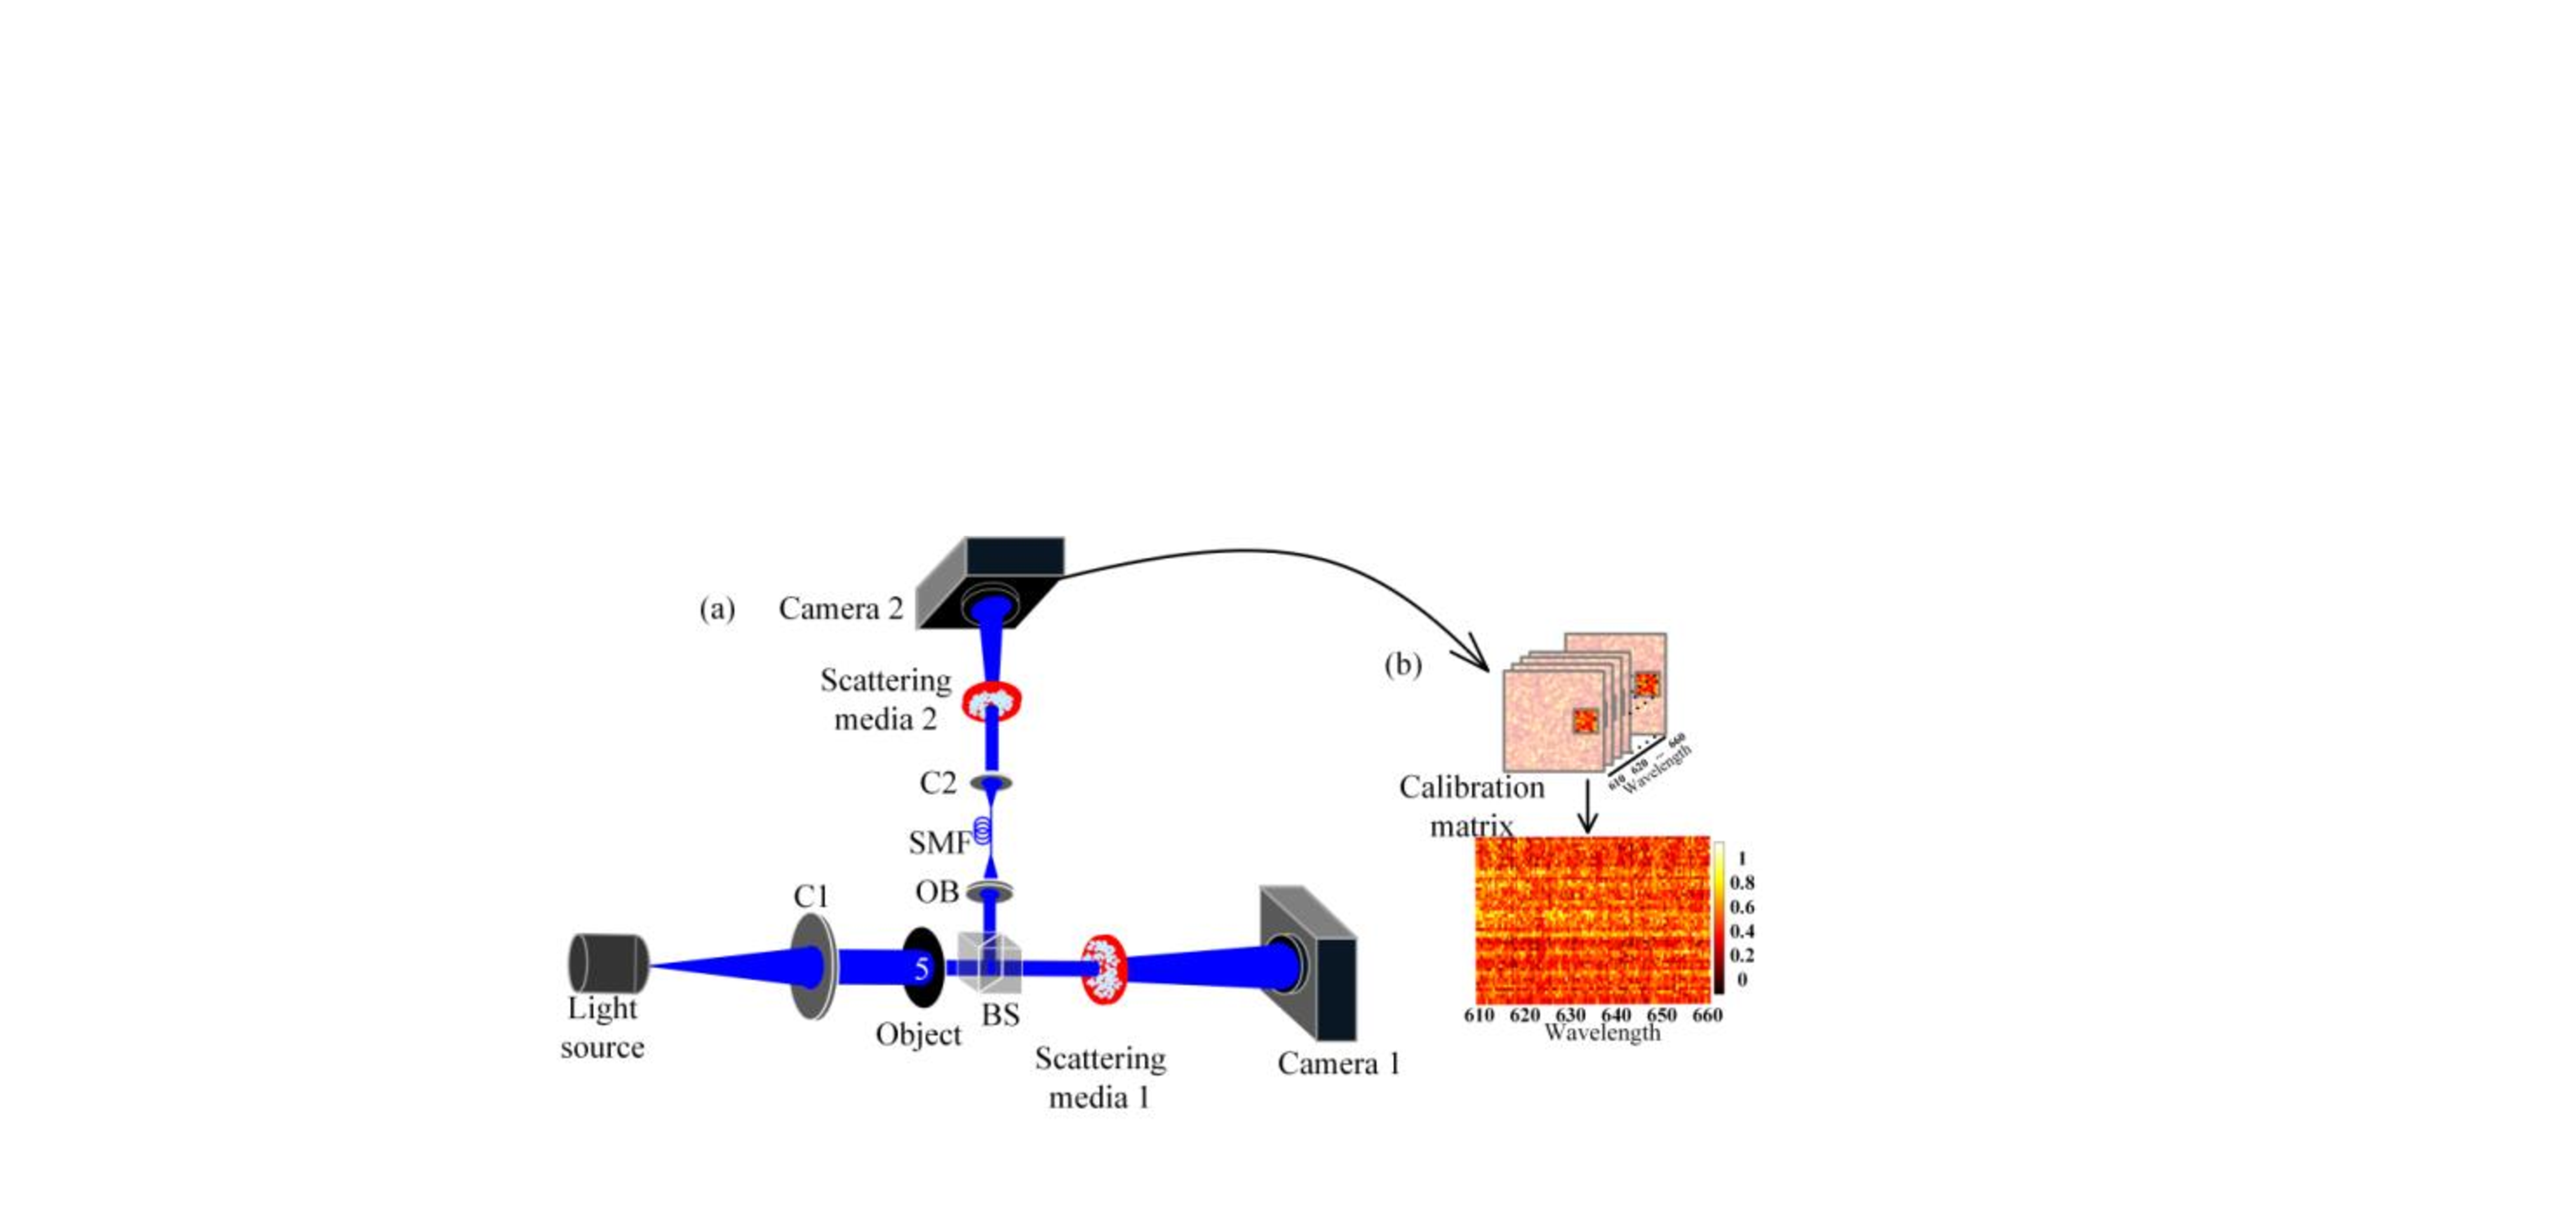
\includegraphics[scale=0.3]{Chapter3.FIG2.spectral_retrieval_model.pdf}
	\caption{透过散射介质的光谱信息和结构信息恢复的结构示意图}
	\label{fig:3.1}
\end{figure}

\subsection{基于光谱传输矩阵的光谱重建模型}
散斑图像中的强度分布取决于照明的角度、观察角度和入射光的波长等因素。在本小节中,我们只对入射光的波长变化进行讨论。首先,我们需要引入散斑的光谱多样性概念。如图\ref{fig:3.2}所示的系统中,照明光源与散射介质之间的距离为$d$,散射介质与相机之间的距离为$S_{0}$,当特定波长以固定的角度照明散射介质时,散射光被位于介质后表面距离为$S_{0}$相机接收。在此,我们认为此类散射介质的散射效应随着波长的改变而变化。我们在惠更斯-菲尼尔近似条件下,相机所接收的散斑图像可以表示为:
\begin{equation}
    E(r_{c},\lambda) = A\iint E(r_{o},\lambda)e^{\frac{ik}{2d}(r_{s}-r_{o})^{2}}Pup.(r_{s},\lambda)T(r_{s},\lambda)e^{\frac{ik}{2S_{o}}(r_{c}-r_{s})^{2}}\mathrm{d}{r_{o}}\mathrm{d}{r_{s}}
\label{eq:wavelength_diversity},
\end{equation}

其中,$k =2\pi/\lambda$,$r_{c}$、$r_{o}$和$r_{s}$分别表示相机平面,光入射面和散射介质平面的坐标,$Pup.(r_{s},\lambda)$为散射介质的孔径函数,$T(r_{s},\lambda)$为介质的散射作用。

我们固定公式(\ref{eq:wavelength_diversity})中的除波长以外参数,分析波长改变对散斑分布的影响。首先,我们假设散射介质对于不同波长光引起的相位变化相同。在此假设下,波长的改变,会引起散斑图案的
空间缩放。其次,对于散射介质来说,其散射效应取决于波长。换而言之,对于不同波长入射光由散射介质引起的相位畸变不同,这样会导致所接受散斑图案分布发生变化,而非简单的缩放。但是对于实际应用中,往往两种
效应同时存在,或者往往更复杂,此种效应被称为散斑的波长多样性。同时我们也进行了相应的仿真,分析波长改变引起的散斑之间的相关系数的改变,仿真结果如图\ref{fig:3.3}所示。如何有效地利用散斑的波长多样性,将对散斑的波长信息利用有着重要的意义。

\begin{figure}[htp]
	\centering
	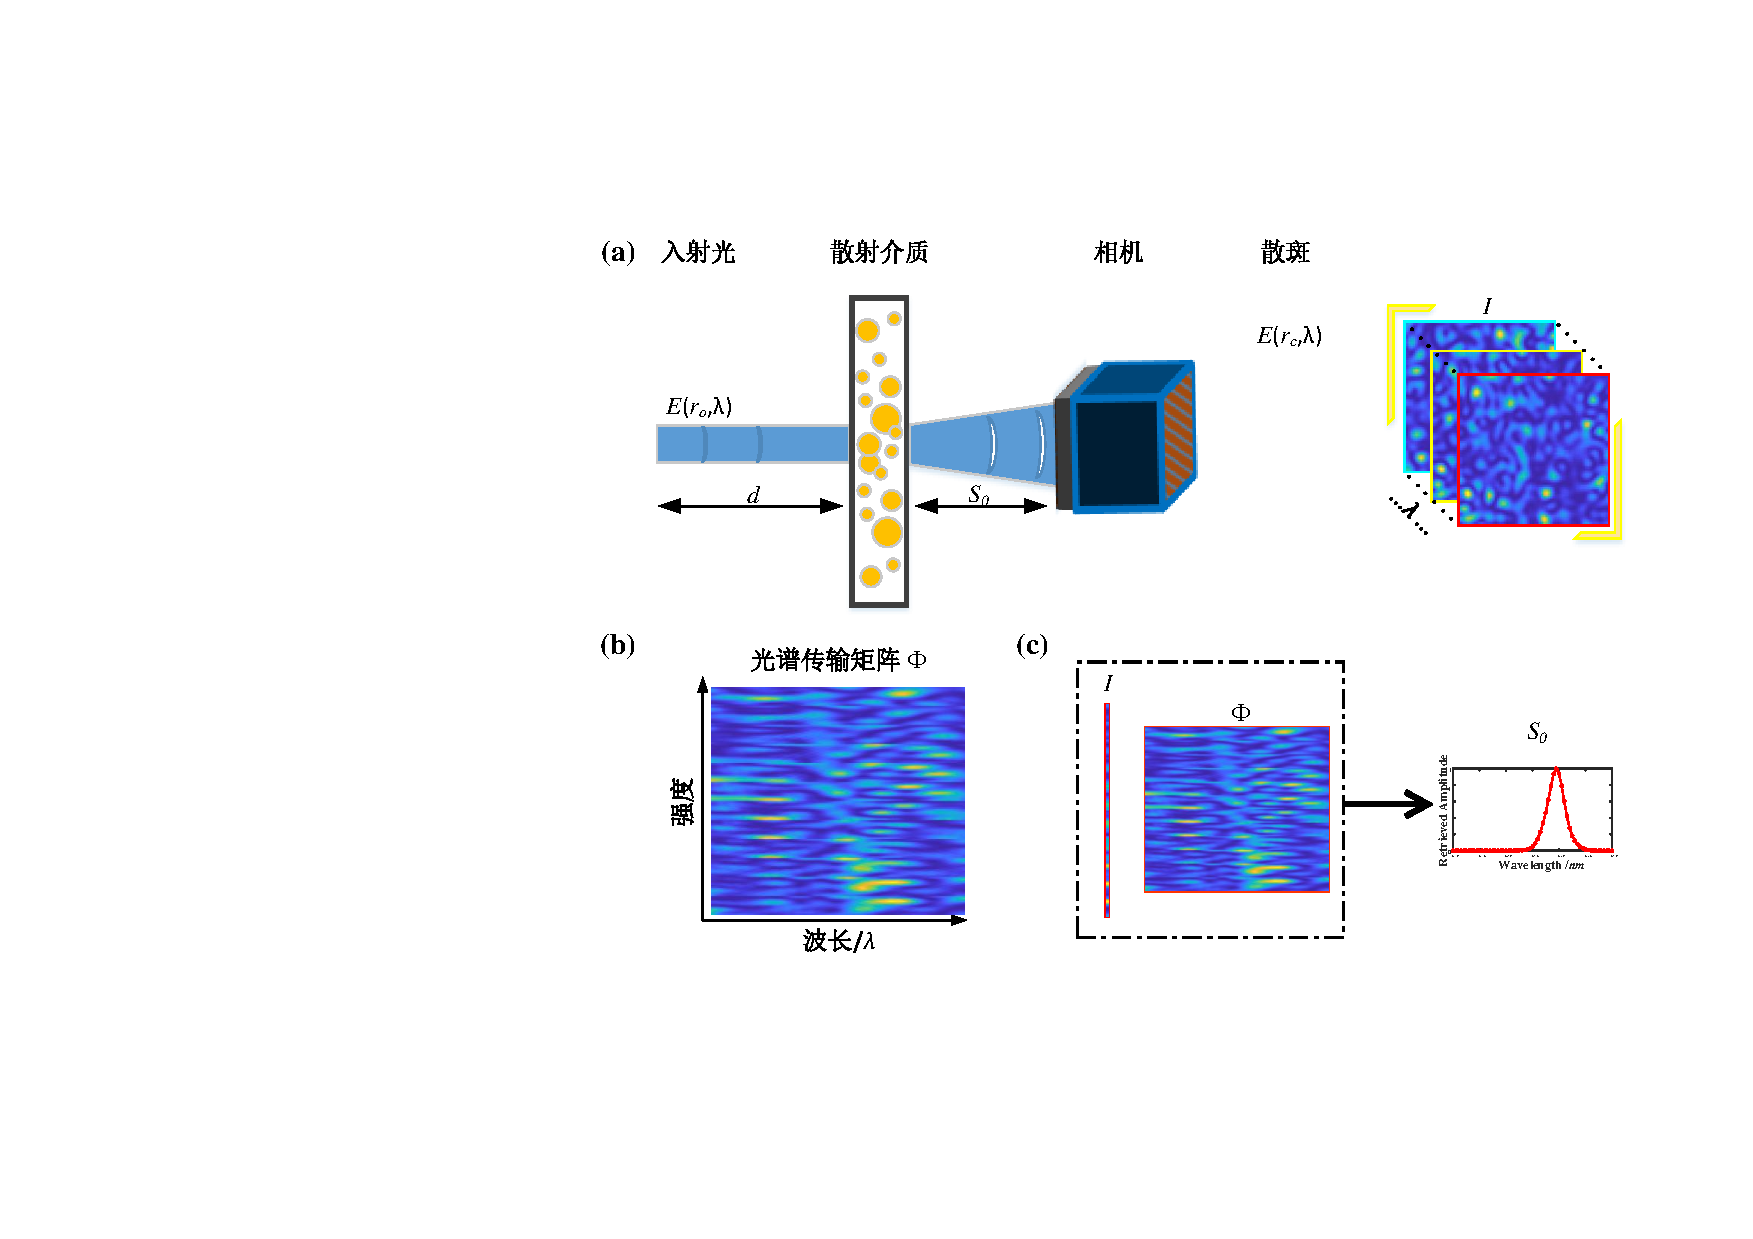
\includegraphics[scale=0.8]{C3.fig13.spectral_retrieval_model.pdf}
	\caption{基于光谱传输矩阵的光谱重建基本原理}
	\label{fig:3.2}
\end{figure}

如果我们对散射介质的光谱指纹进行标定,并将不同的光谱指纹存储在矩阵中,此矩阵称为光谱传输矩阵。在此情况下,在获得未知光源照射散射介质所获得的散斑后,是否能够光谱传输矩阵和此散斑对未知光源的光谱信息进行重建?答案是可以。如图\ref{fig:3.1}b所示,将不同的光谱指纹转换行向量,并按照光谱信息存储在矩阵$\Phi$中,当获取未知光源对应的散斑时,同样将其转换为向量$I$。所以,其输入信号的光谱$S$可以表示为:$I={\Phi}S$,对矩阵进行左乘求逆,并求出最小二乘解:$S={\Phi}^{-1}I$。值得强调的是,该光谱重建方法不仅局限于对于以标定的单色光谱信号进行重建,同时也可应用于连续光谱信号。上述的光谱重建问题可转化为更普遍的最小化问题:$s_{0}=\arg{\min_s \| I -{\Phi}S \|_2}$,其中$\| \cdot \|_2$表示$L_2$范数,$s_{0}$表示所重建的光谱信号,可以通过采用不同的最小化优化算法解决此问题。
\begin{figure}[htp]
	\centering
	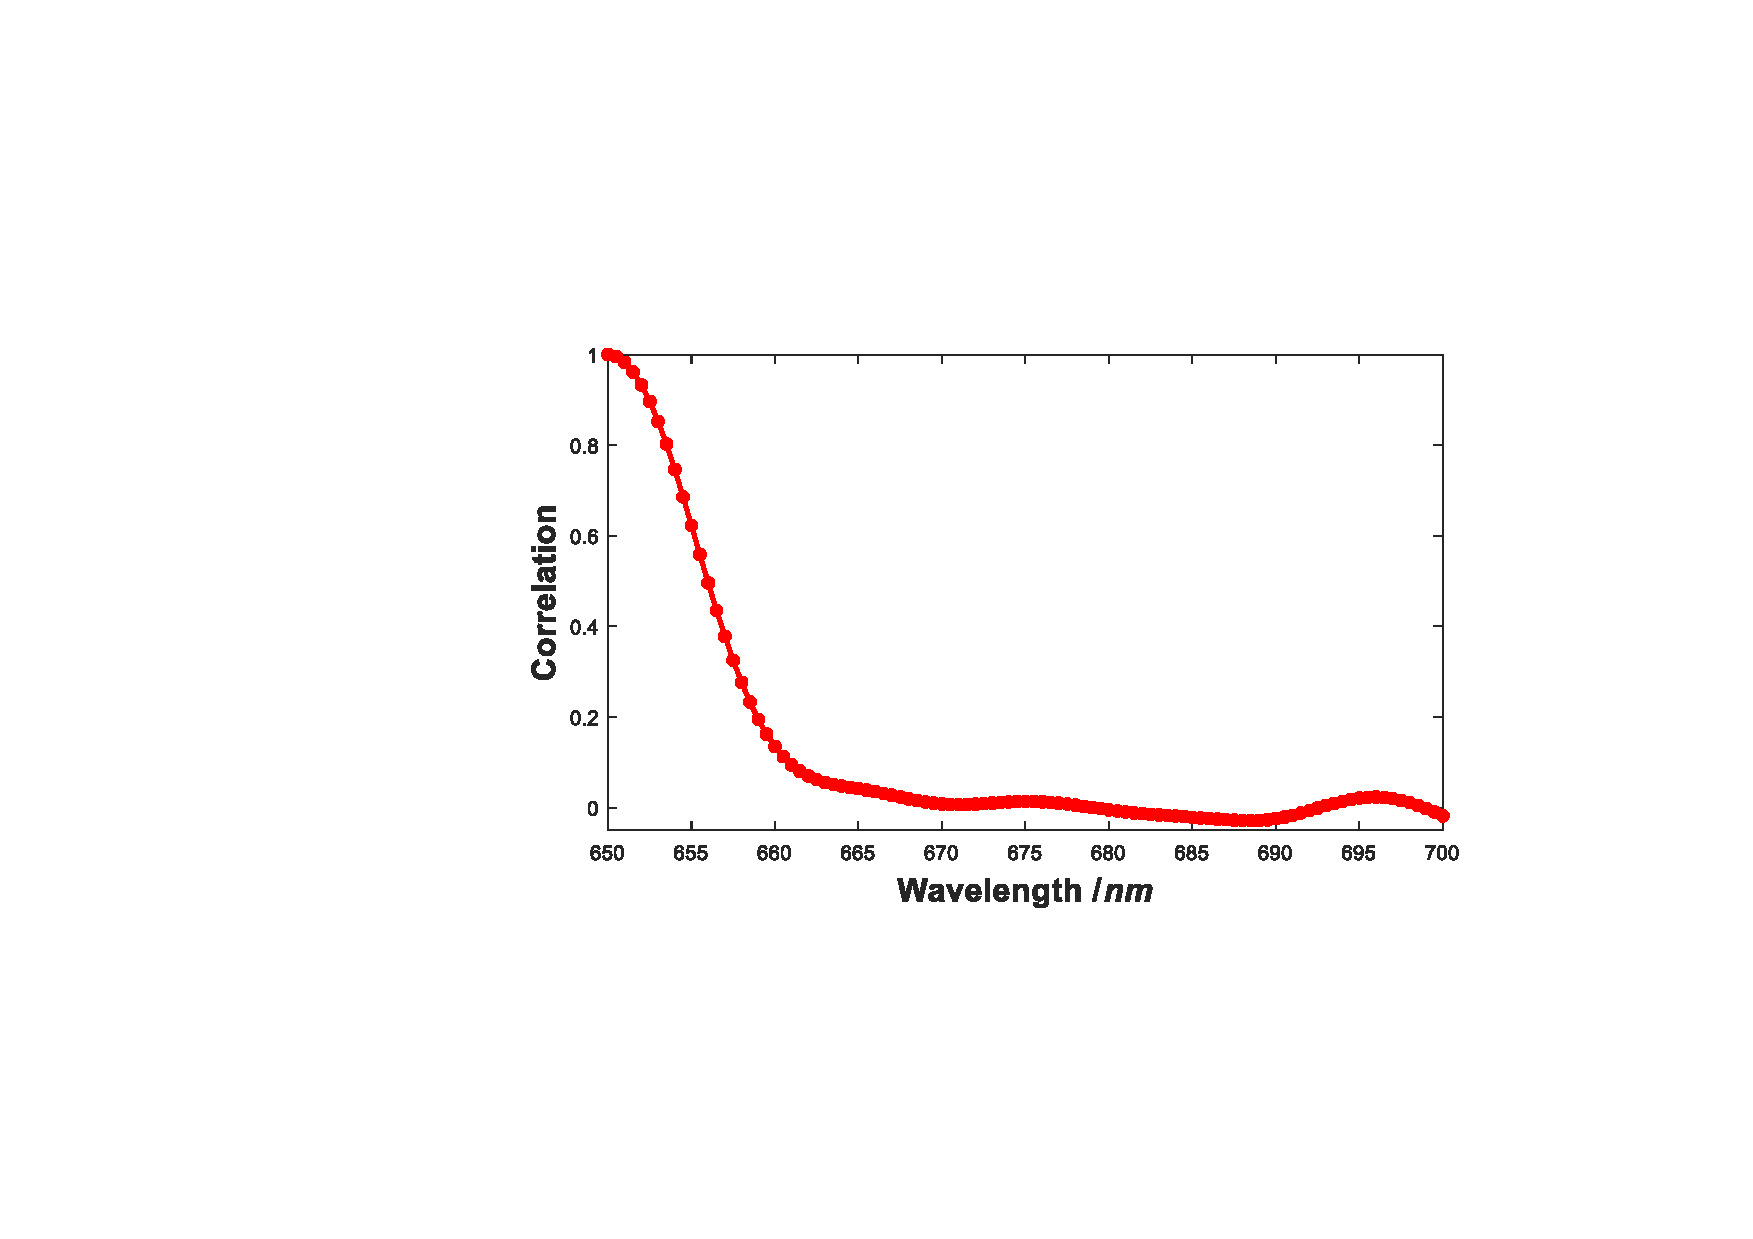
\includegraphics[scale=0.5]{C3.fig3.spectral_correlation_speckle.pdf}
	\caption{散斑的相关系数}
	\label{fig:3.3}
\end{figure}
\subsection{基于OME的散斑相关成像模型}
图\ref{fig:3.4}所示为基于光学记忆相应的散斑相关成像基本模型,目标与散射介质之间的距离为$d$,散射介质与相机之间的距离为$S_{0}$。目标由空间非相干光源照明提供照明,目标所发出的光经过散射介质后,被相机所接收。当物体位于此散射介质的OME范围之类时,由于OME范围内的PSF具有空间平移不变性,相机所探测到的散斑可以表示为:
\begin{figure}[htp]
	\centering
	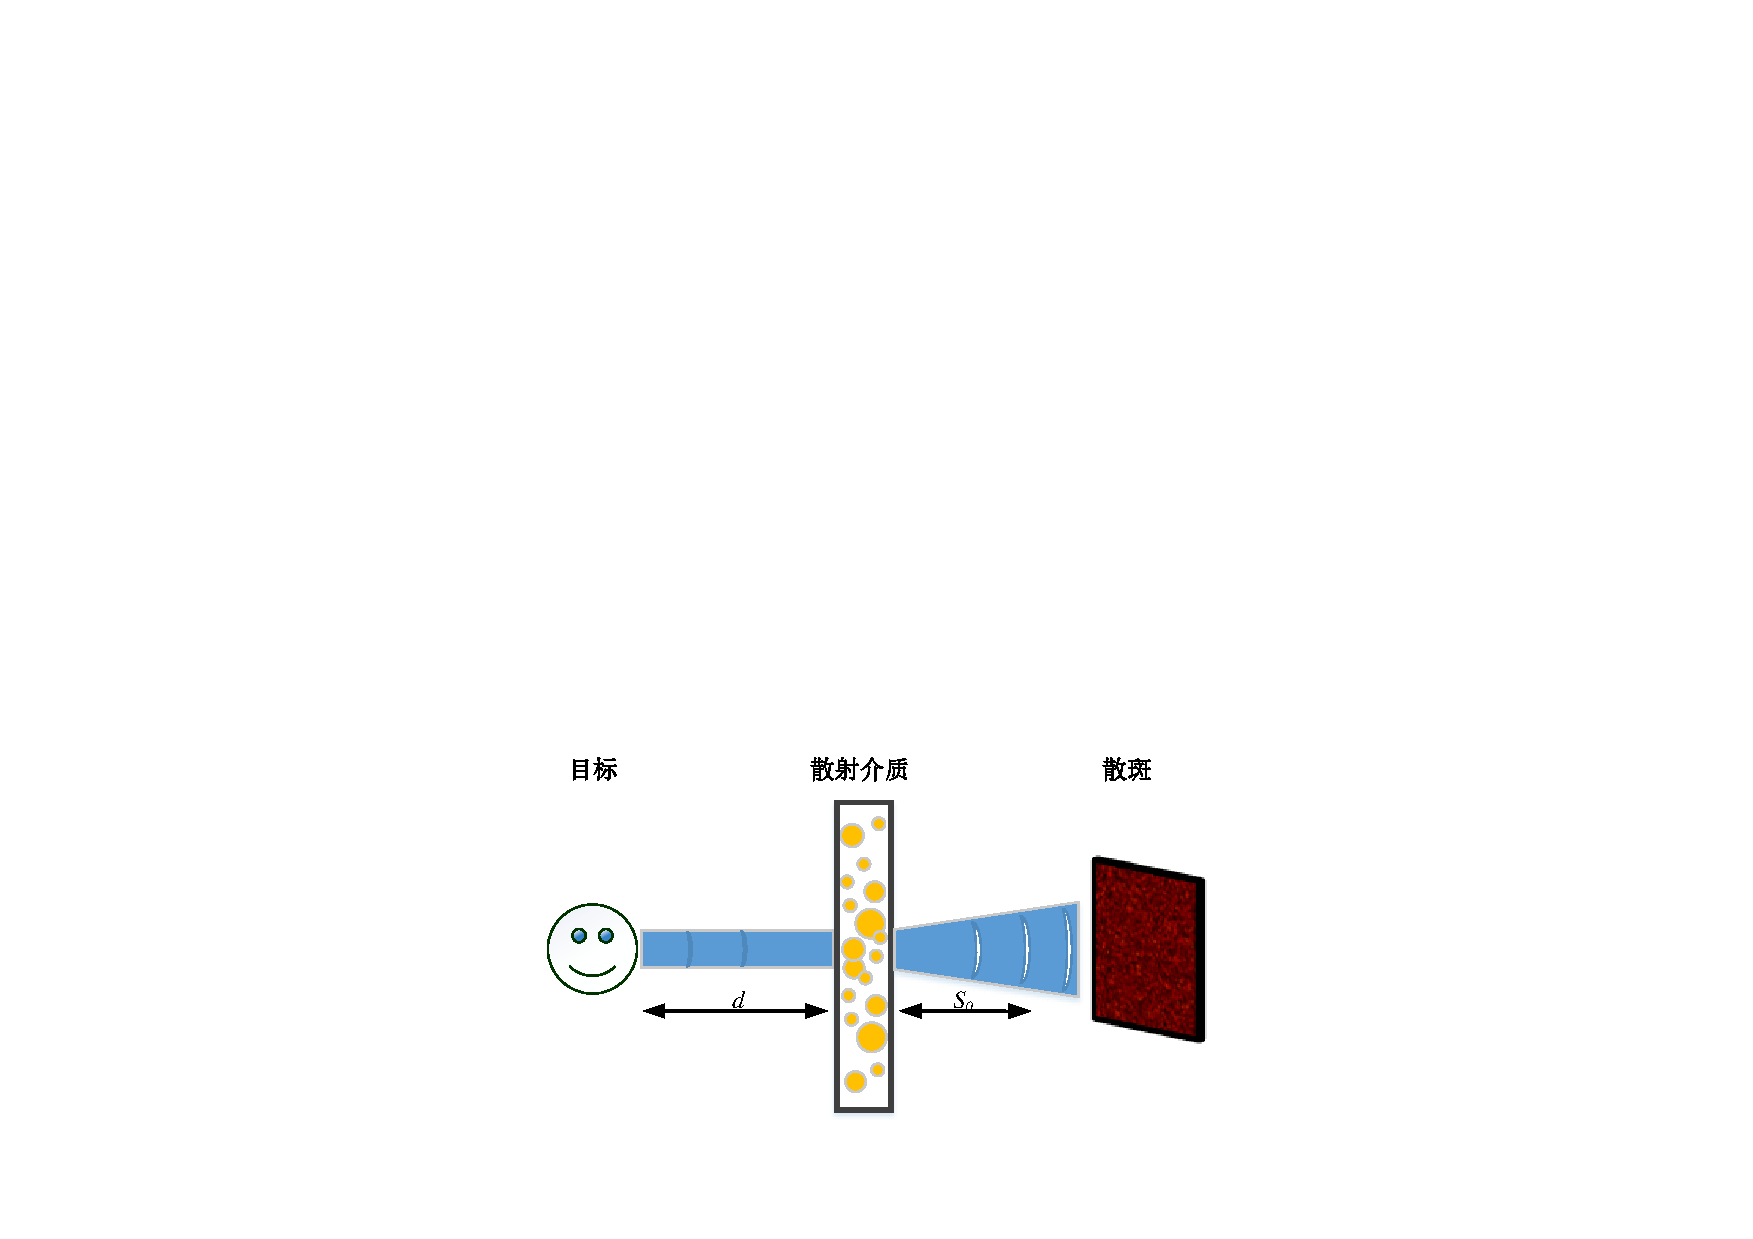
\includegraphics[scale=0.7]{C3.fig4.imaging_model.pdf}
	\caption{散斑相关成像模型}
	\label{fig:3.4}
\end{figure}

\begin{equation}
    I = O*S
\label{eq:speckle_autocorrelation_imgaing}
\end{equation}其中,$*$为卷积运算,$I$表示相机散斑,$O$表示目标和$S$表示系统的PSF。

透过散射成像的数学模型的理论基础如下,目标可以分解为不同的点源目标,当不同的点源目标为与散散介质的OME范围之内时,不同点源目标所对于系统的响应函数可以近似看作不同的散斑在空间的平移。假设所有的点源目标被同时点亮时,相机所接收到的图像为不同点源目标所对应散斑的非相干叠加。所以,OME范围内目标的非相干成像模型可以卷积的形式进行表示:$I = O*S$。但是值得注意的是,大多是散射介质的OME范围是有限的,当目标的尺寸超过OME范围时,此时卷积模型需要加入新的限制条件。成像系统的放大率$M$取决于物距$d$和相距$S_{0}$:
\begin{equation}
    M = \frac{d}{S_{0}}
\label{eq:magnification_imgaing_system}
\end{equation}
成像系统的分辨率$\Delta \theta $可以表示为:
\begin{equation}
    \Delta \theta   \propto \frac{\lambda}{nD}
\label{eq:angleresolution_imgaing_system}
\end{equation}
其中,$\propto$表示正比关系,$\lambda$为照明光源的波长,$n$表示光经过散射介质后的介质折射率,$D$表示散射介质的有效孔径,孔径的大小可以通过加载光阑实现控制。

上述部分中,我们具体描述了基于OME的散射基本成像模型,如公式(\ref{eq:speckle_autocorrelation_imgaing})所示,当获得散斑图像后如何恢复图像将在接下来部分进行描述。意大利学者J.Bertolotti,以色列学者O.Katz等人先后基于散斑自相关的特性,提出了基于光学散斑自相关的图像重建算法。当相机获得散斑图案后,散斑的自相关可以表示为:
\begin{equation}
\begin{aligned}
    I \bigstar I  &= (O*S) \bigstar (O*S) \\
		              &=  (O \bigstar O)*(S \bigstar S)
\end{aligned}
\label{eq:autocorelation_equation}
\end{equation}
其中,$\bigstar$表示自相关运算。由公式(\ref{eq:autocorelation_equation})可知,散斑的自相关可以表示为目标的自相关与系统PSF自相关的卷积。当前成像系统PSF的自相关$(S \bigstar S)$可以近似为$\delta$函数。所以,公式(\ref{eq:autocorelation_equation})可以简化为:
\begin{equation}
\begin{aligned}
    I \bigstar I  = (O \bigstar O)+C
\end{aligned}
\label{eq:autocorelation_equation_1}
\end{equation}
其中,$C$表示自相关计算中的背景常数项。通常,在自相关图像恢复中,我们需要将背景常数项进行剔除。如果对公式(\ref{eq:autocorelation_equation_1})左右两边同时进行傅里叶变换,我们会获得什么呢?庆幸的是,我们获得了以下公式:
\begin{equation}
\begin{aligned}
    \mathcal{F}(I \bigstar I)  = \mathcal{F}(O \bigstar O)
\end{aligned}
\label{eq:autocorelation_equation_2}
\end{equation}
公式(\ref{eq:autocorelation_equation_2})继续可以简化为:
\begin{equation}
\begin{aligned}
    \mid \mathcal{F}(O) \mid = \sqrt{\mathcal{F}(O \bigstar O)}\\
		               = \sqrt{\mathcal{F}(I \bigstar I)}
\end{aligned}
\label{eq:autocorelation_equation_3}
\end{equation}
根据公式(\ref{eq:autocorelation_equation_3})可知,我们可以通过计算的方式从散斑图像中获得隐藏目标的傅里叶振幅信息,当获得目标的傅里叶振幅信息之后,仍然缺失的是目标的傅里叶相位信息。图像恢复问题已经被转换为依据傅里叶振幅信息恢复傅里叶相位信息的问题,幸运的是此类相位恢复问题在相位中属于常见问题。相位恢复算法不是本节研究的重点,因此在本节中,我们将简要介绍在后续图像恢复中所用到的基本相位恢复算法,其算法流程如图\ref{fig:3.5}所示。该类型相位算法的核心思想为:步骤一,获得傅里叶振幅信息$\mid \mathcal{F}(O) \mid$,随机的给予随机的傅里叶相位初始值$\phi$,并对其进行傅里叶变换,进而将信号转换至空间域,并获得目标的初始猜测$g_t(x,y)$;步骤二,对信号$g_t(x,y)$进行傅里叶变换,将其变换至频域$G_t(k_x,k_y)$,将$G_t(k_x,k_y)$的傅里叶振幅部分替换为$\mid \mathcal{F}(O) \mid$,保留其傅里叶相位信息,此时的信号表示为$G^{\prime}_t(k_x,k_y) =\mid \mathcal{F}(O) \mid e^{i\phi (k_x,k_y)}$;步骤三,对信号$G^{\prime}_t(k_x,k_y)$进行再一次傅里叶变换,将其转换至空间域,根据目标信号的稀疏性及非负性,设置约束条件,对信号进行处理,此时获得的信号表示为:$g^{\prime}_t(x,y)$;步骤四,用$g^{\prime}_t(x,y)$替换为步骤一中的$g_t(x,y)$,并重复步骤二至步骤四,直至满足约束条件停止此相位恢复程序。

\begin{figure}[htp]
	\centering
	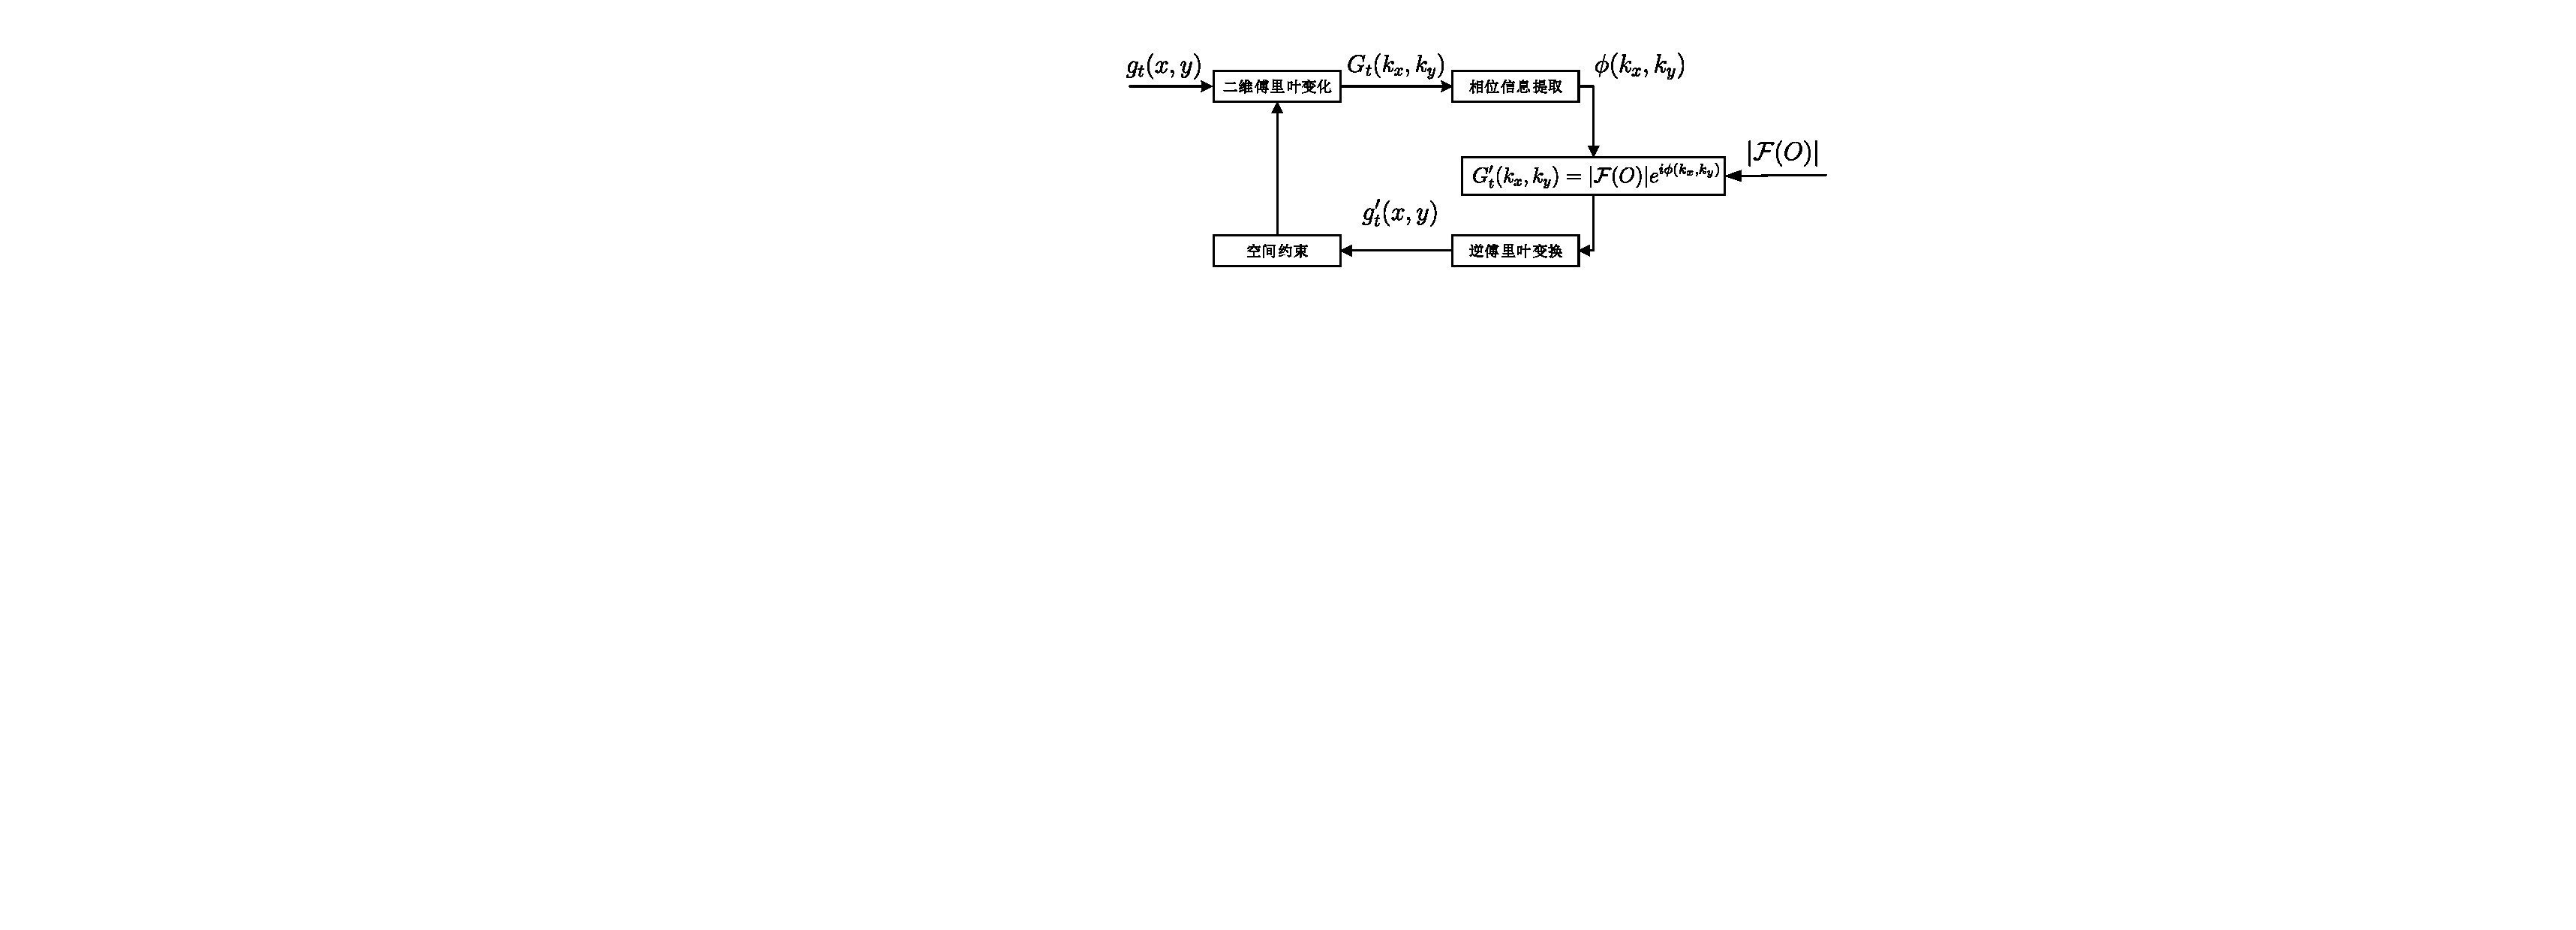
\includegraphics[scale=0.7]{C3.fig5.phase_retrieval_model.pdf}
	\caption{基本相位恢复流程图}
	\label{fig:3.5}
\end{figure}
在实际的应用中,不同相位恢复算法在空间域采用不同的约束条件。例如,混合输入输出(Hybrid Input-Output,HIO)算法的约束条件如公式(\ref{eq:constrain_HIO})所示,误差减小(Error reduction,ER)算法的约束条件如公式如公式(\ref{eq:constrain_ER})所示。
\begin{equation}
\begin{aligned}
 g_{t+1}(x,y) =
		  \begin{cases}
		    g_{t}^{\prime}(x,y)   &   (x,y)\notin\Gamma\\
		    g_{t}(x,y)-\beta g_{t}^{\prime}(x,y) & (x,y)\in\Gamma
		  \end{cases}
\end{aligned}
\label{eq:constrain_ER}
\end{equation}
其中,$\beta$为算法收敛性的参数,$\Gamma$为满足约束条件的集合。

\begin{equation}
\begin{aligned}
 g_{t+1}(x,y) =
		  \begin{cases}
		    g_{t}^{\prime}(x,y)   &   (x,y)\notin\Gamma\\
		    0  & (x,y)\in\Gamma
		  \end{cases}
\end{aligned}
\label{eq:constrain_HIO}
\end{equation}

\section{光谱信息恢复及散斑自相关成像方法仿真验证}\label{光谱传输矩阵章节}
上述部分,我们对光谱信息恢复及散斑相关成像的基本原理继续了介绍,因此在本小节中,我们对上述的原理进行数字仿真验证及实验验证。
B.Redding等人在文献中以对基于光谱传输矩阵的光谱重建方法进行了详细的理论分析,所以在此我们对该方法进行简单的数值分析以及仿真验证。光谱重建的仿真原理如图\ref{fig:3.2}所示,
分别记录不同波长输入光对应的散斑$I_\lambda$,并将$I_\lambda$存储在光谱传输矩阵中。然后,输入未知光谱$s_{o}$记录其对应的散斑信号$I_{o}$,根据公式$s_{0}=\arg{\min_s \| I_{o} -{\Phi}S \|_2}$对光谱$s_{0}$进行求解。
在散斑图像重建方面,首先我们生成对应的PSF,根据公式(\ref{eq:speckle_autocorrelation_imgaing})生成目标对应的散斑,然后利用上述的散斑自相关成像方法进行图像恢复。

透过散射介质光谱成像的仿真参数如表\ref{table:1.1}所示,仿真结果如图\ref{fig:3.6}所示,第一行,为成像臂在不同波长光照明情况下,相机1所探测到的散斑;第二行,为光谱臂在不同光谱不同波长光照明下,相机2所接收到的散斑;
第三行,利用散斑相关成像方法所恢复的目标图像;第四行,利用光谱传输矩阵方法所恢复的光谱信息。从仿真结果图\ref{fig:3.6}第一列至第三列可以看出,当输入光为窄带宽的光源时,该光谱成像方法能够有效地恢复图标的空间信息和光谱信息。从图\ref{fig:3.6}第四列可以看出,当照明光源为宽谱光源时,该光谱成像方法仍然能够有效的重建目标的光谱信息和空间信息。

\begin{table}[htp]
\begin{center}
\caption{仿真参数}
\label{table:1.1}
\begin{tabular}{|c|c|}
\hline
\textbf{仿真参数} & \textbf{数值}\\
\hline
光谱范围 & $600 \sim 650 nm$ \\
\hline
光谱采样间隔 & $0.5  nm$\\
\hline
空间采样间隔 & $12.0 \mu m$ \\
\hline
散射介质维度 & $600 \times 600$ \\
\hline
\end{tabular}
\end{center}
\end{table}

我们所用到的基于光谱传输矩阵的光谱重建方法对于系统的噪声叫敏感,不同的重建优化方法在抗噪声方面有着不同表现。于是,我们通过在系统中引入不同功率的高斯噪声,并且进行了相应的重建,计算重建信号与原始信号之间的相关系数,进而分析不同算法的抗噪性能。目前常用的重建算法有:吉洪诺夫正则化算法(Tikhonov regularization,TR)和凸优化算法(Convex Optimization,CVX),TR和CVX重建算法在不同噪声水平下的光谱重建结果如图\ref{fig:3.7}所示。从图\ref{fig:3.7}中看可以看出,随着噪声从$50 dB$ 增加到 $35 dB$,TR和CVX两种重建算法的分别重建的光谱信号与原始信号之间相关系数接近于1,但是当信噪比低于 $35 dB$时,CVX重建结果的相关系数大于TR重建的相关系数。因此我们相信,CVX在光谱重建方面的抗噪性能优于TR。

\begin{figure}[htp]
	\centering
	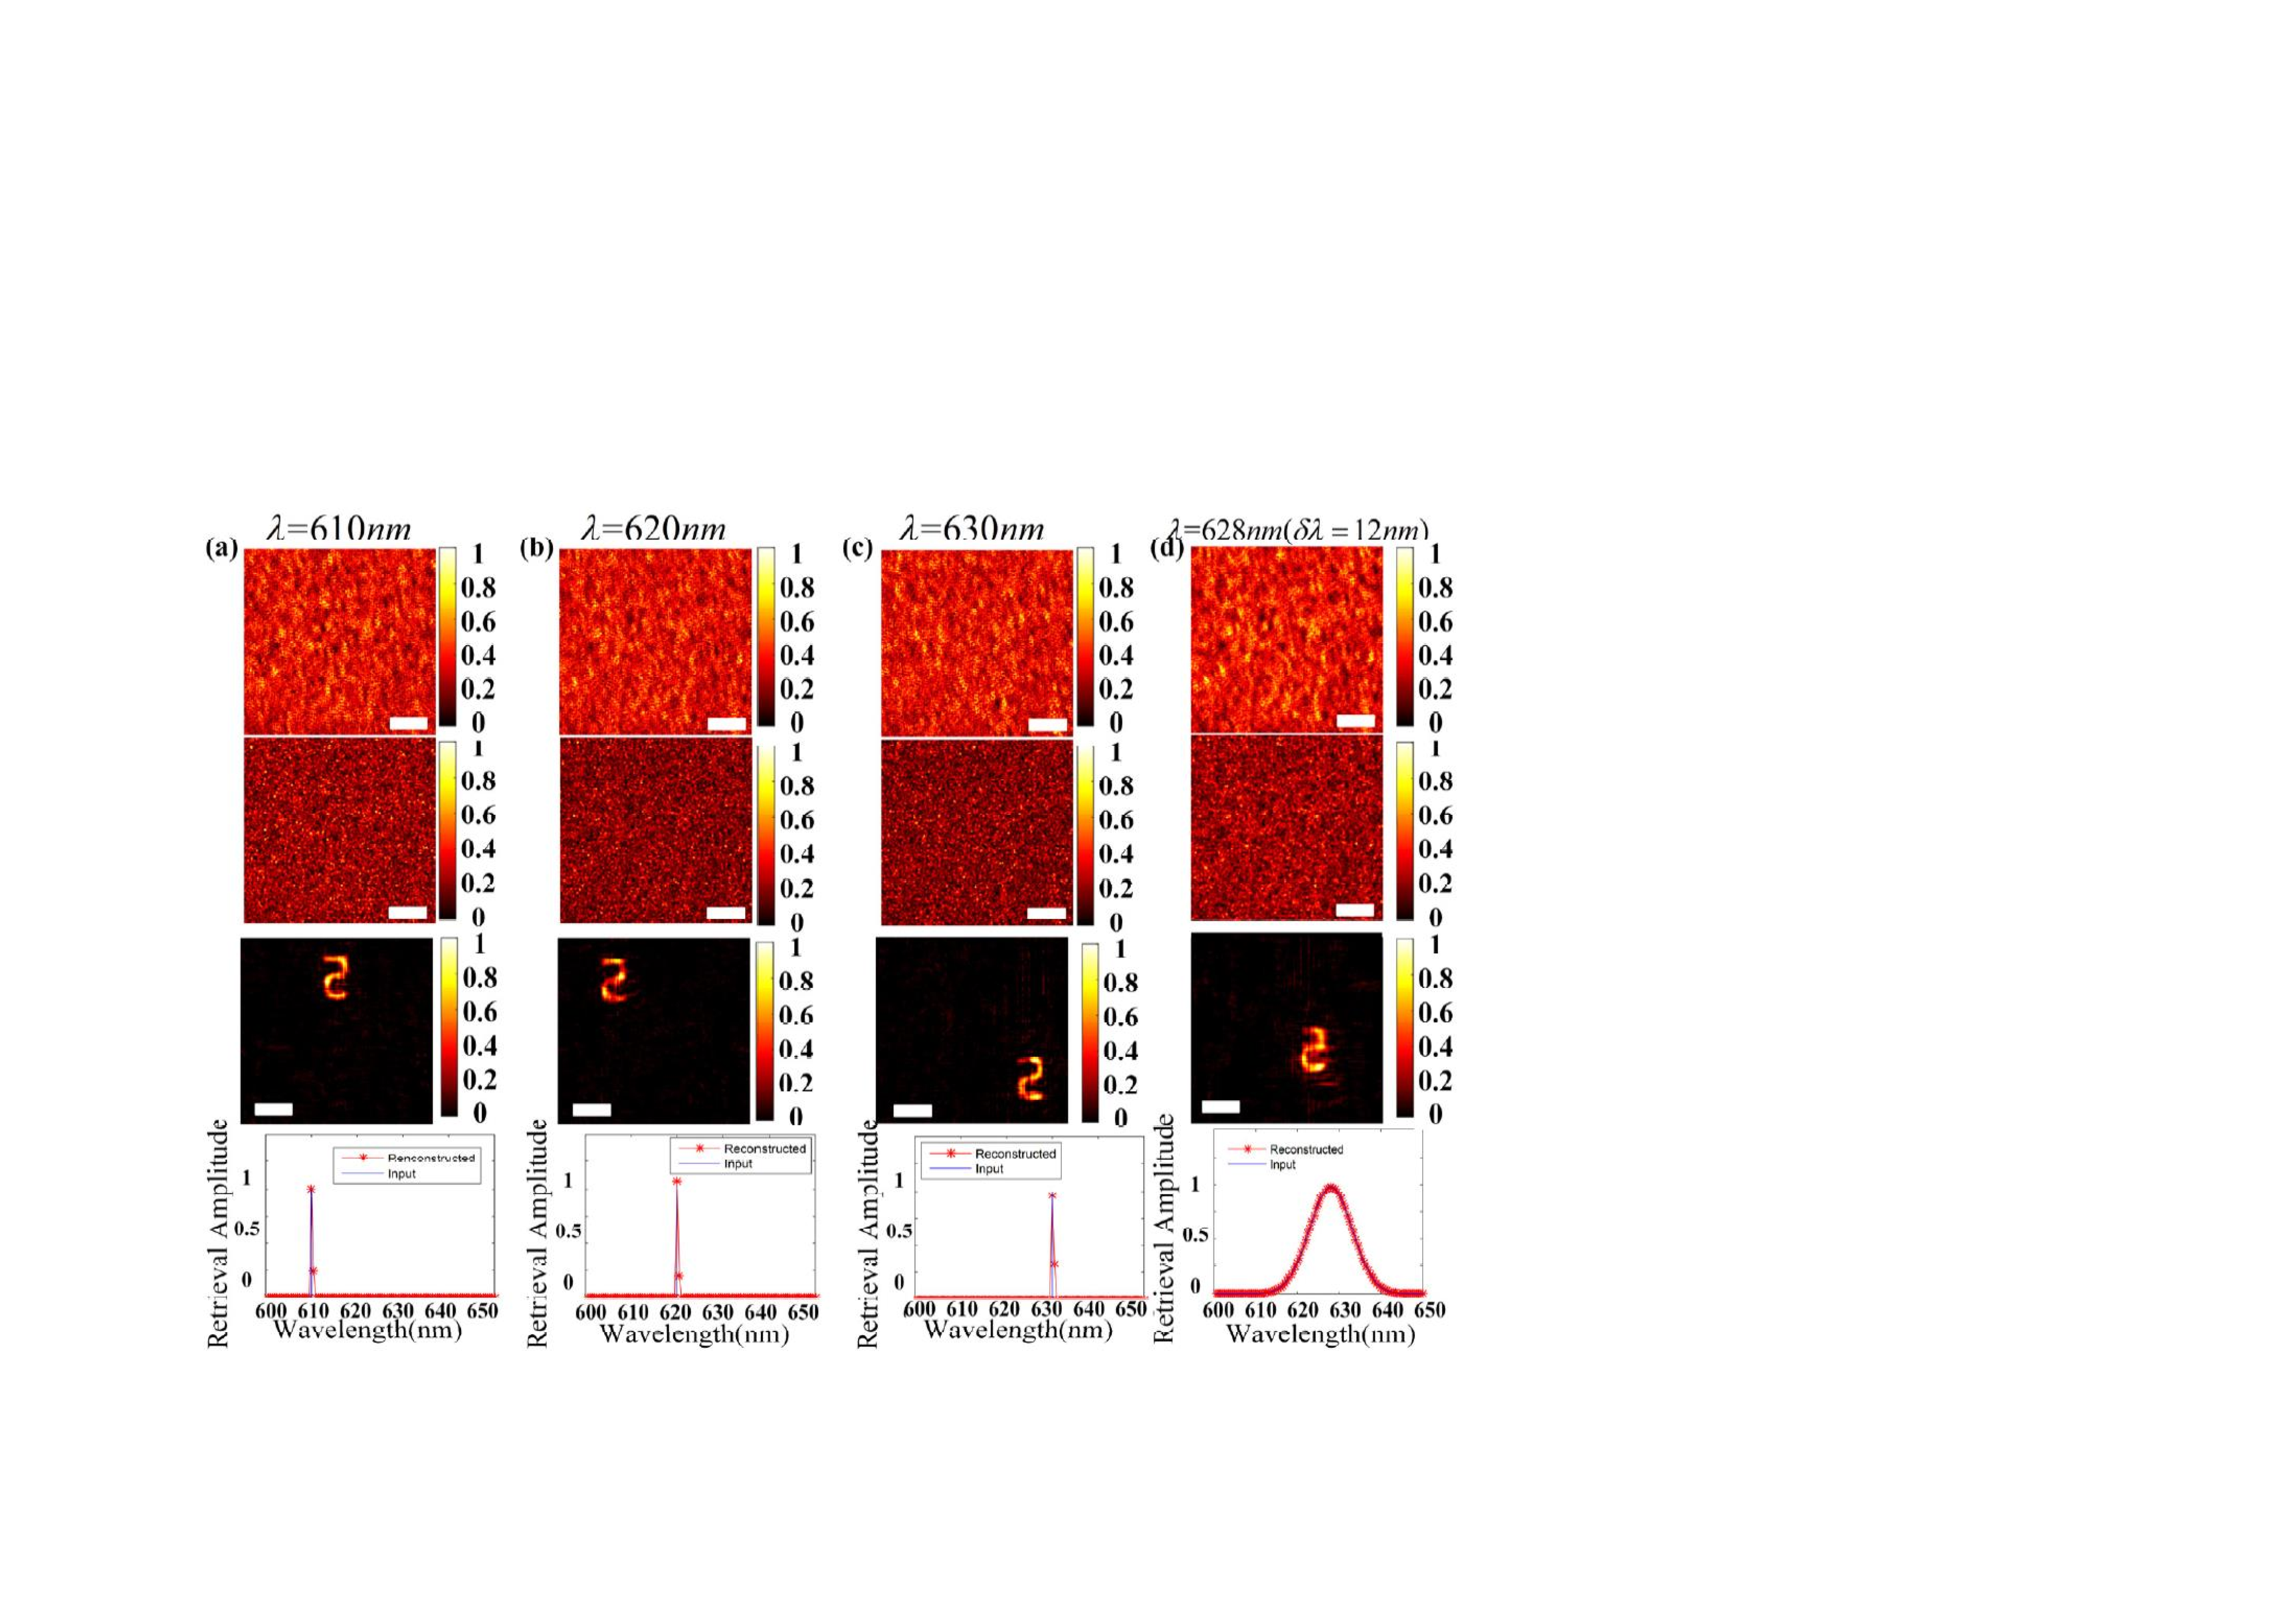
\includegraphics[scale=0.45]{C3.fig6.simulation_results.pdf}
	\caption{仿真结果}
	\label{fig:3.6}
\end{figure}

\begin{figure}[htp]
	\centering
	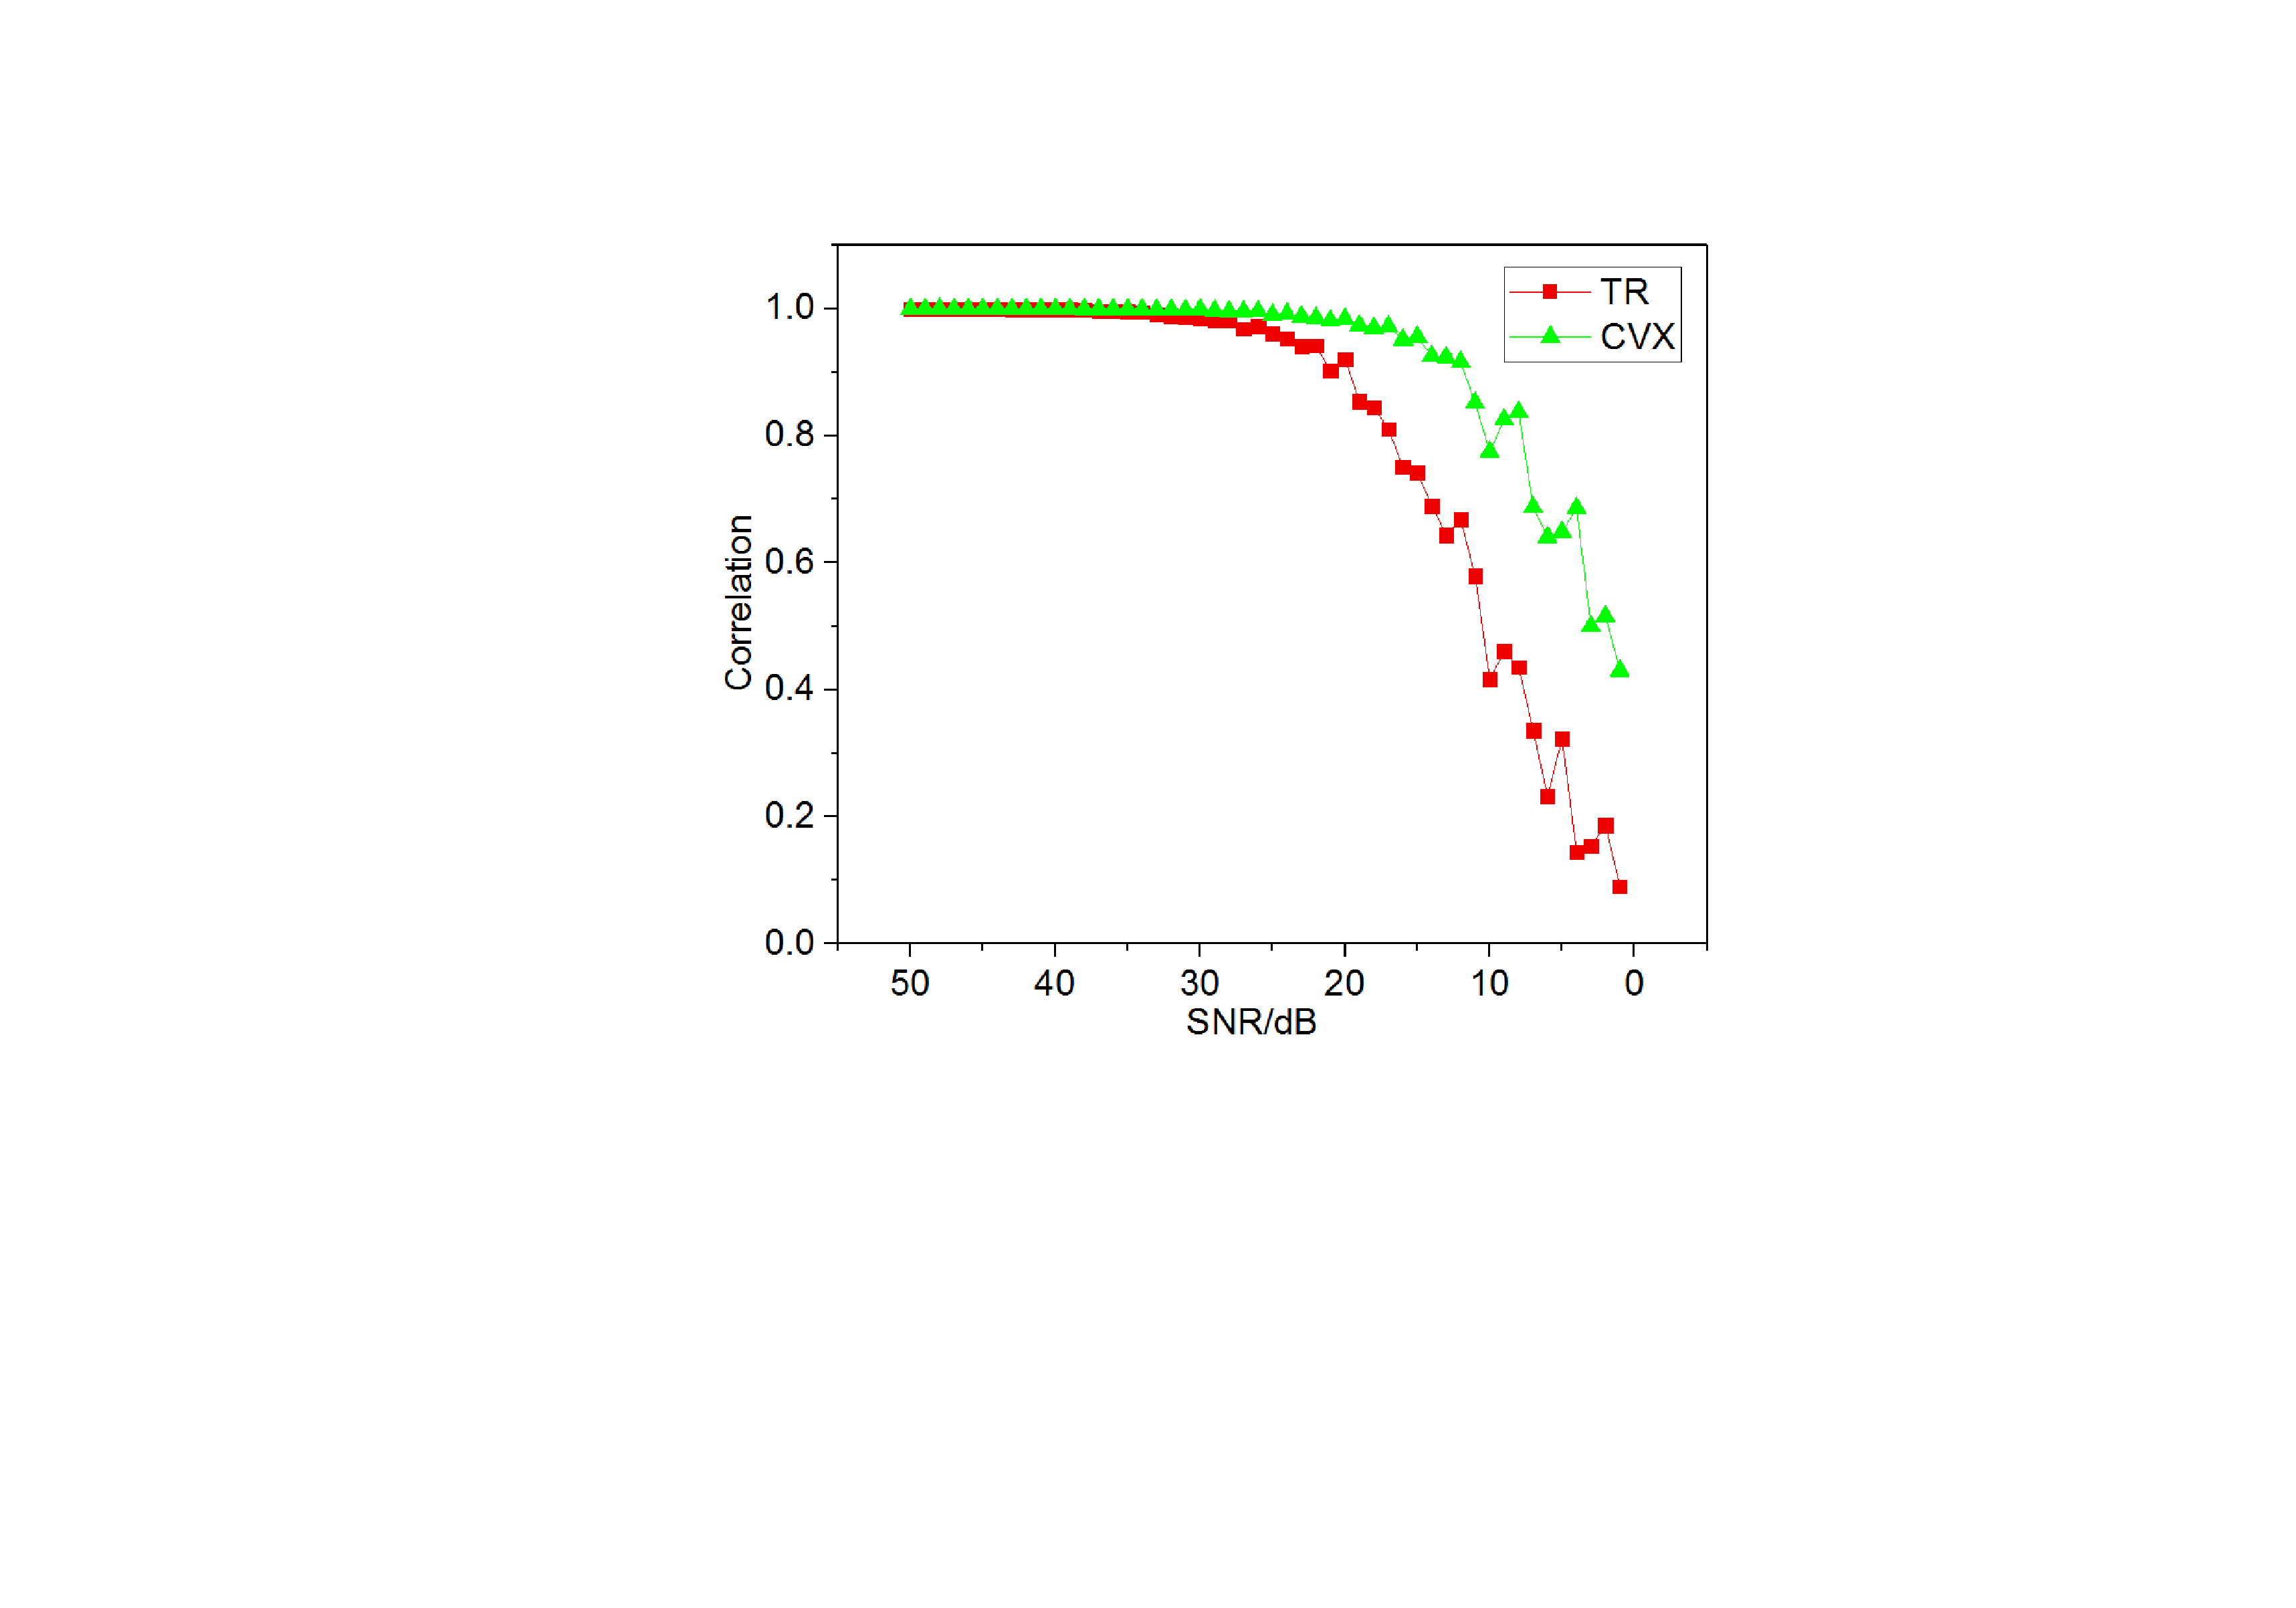
\includegraphics[scale=0.28]{C3.fig7.performance_under_fifferent_noise_levels.pdf}
	\caption{光谱重建算法的抗噪性能分析}
	\label{fig:3.7}
\end{figure}

\section{光谱信息恢复及散斑自相关成像方法实验验证}

实验光学装置如图\ref{fig:3.8}所示,{\large \textcircled{\normalsize 1}}:光源,{\large \textcircled{\normalsize 2}}:单色仪,{\large \textcircled{\normalsize 3}}:准直器,{\large \textcircled{\normalsize 4}}:分束器,{\large \textcircled{\normalsize 5}}:目标,{\large \textcircled{\normalsize 6}}:散射介质1,{\large \textcircled{\normalsize 7}}:相机1,
{\large \textcircled{\normalsize 8}}:物镜,{\large \textcircled{\normalsize 9}}:单模光纤,
{\large \textcircled{\normalsize 10}}:透镜,{\large \textcircled{\normalsize 11}}:散射介质2和{\large \textcircled{\normalsize 12}}:相机2。
在实验中,我们使用厚度为$2mm$,颗粒度为$220$毛玻璃(Thorlabs,DG10-220)作为散射介质,目标为从分辨率测试靶标(1951USAF,Edmund Company)中选出的数字字符。
实验中,我们需要对光谱臂进行预标定,目的是获取光谱臂的光谱传输矩阵。在预标定过程中,我们利用来自氙气灯(Zolix, GLORIA-X500A)的作为照明光源,并用安道尔单色仪(Andor Spectrograph, Shamrock 500i)对照明光源进行光谱过滤,产生光谱分辨率,即全宽半高
(Full Width Half Maximum,FWHM),为$1 nm$的可调光源。实验中使用相机是CMOS相机(AndorZyla5.5),像素尺寸为$6.5\mu m$和像素数为420万。
实验中,我们分别对$445 \sim 495nm$ 和 $610 \sim 660nm$两个光谱波段进行标定,预标定后的光谱传输矩阵分别如图\ref{fig:3.8}(b)和\ref{fig:3.8}(c)所示。

\begin{figure}[htp]
	\centering
	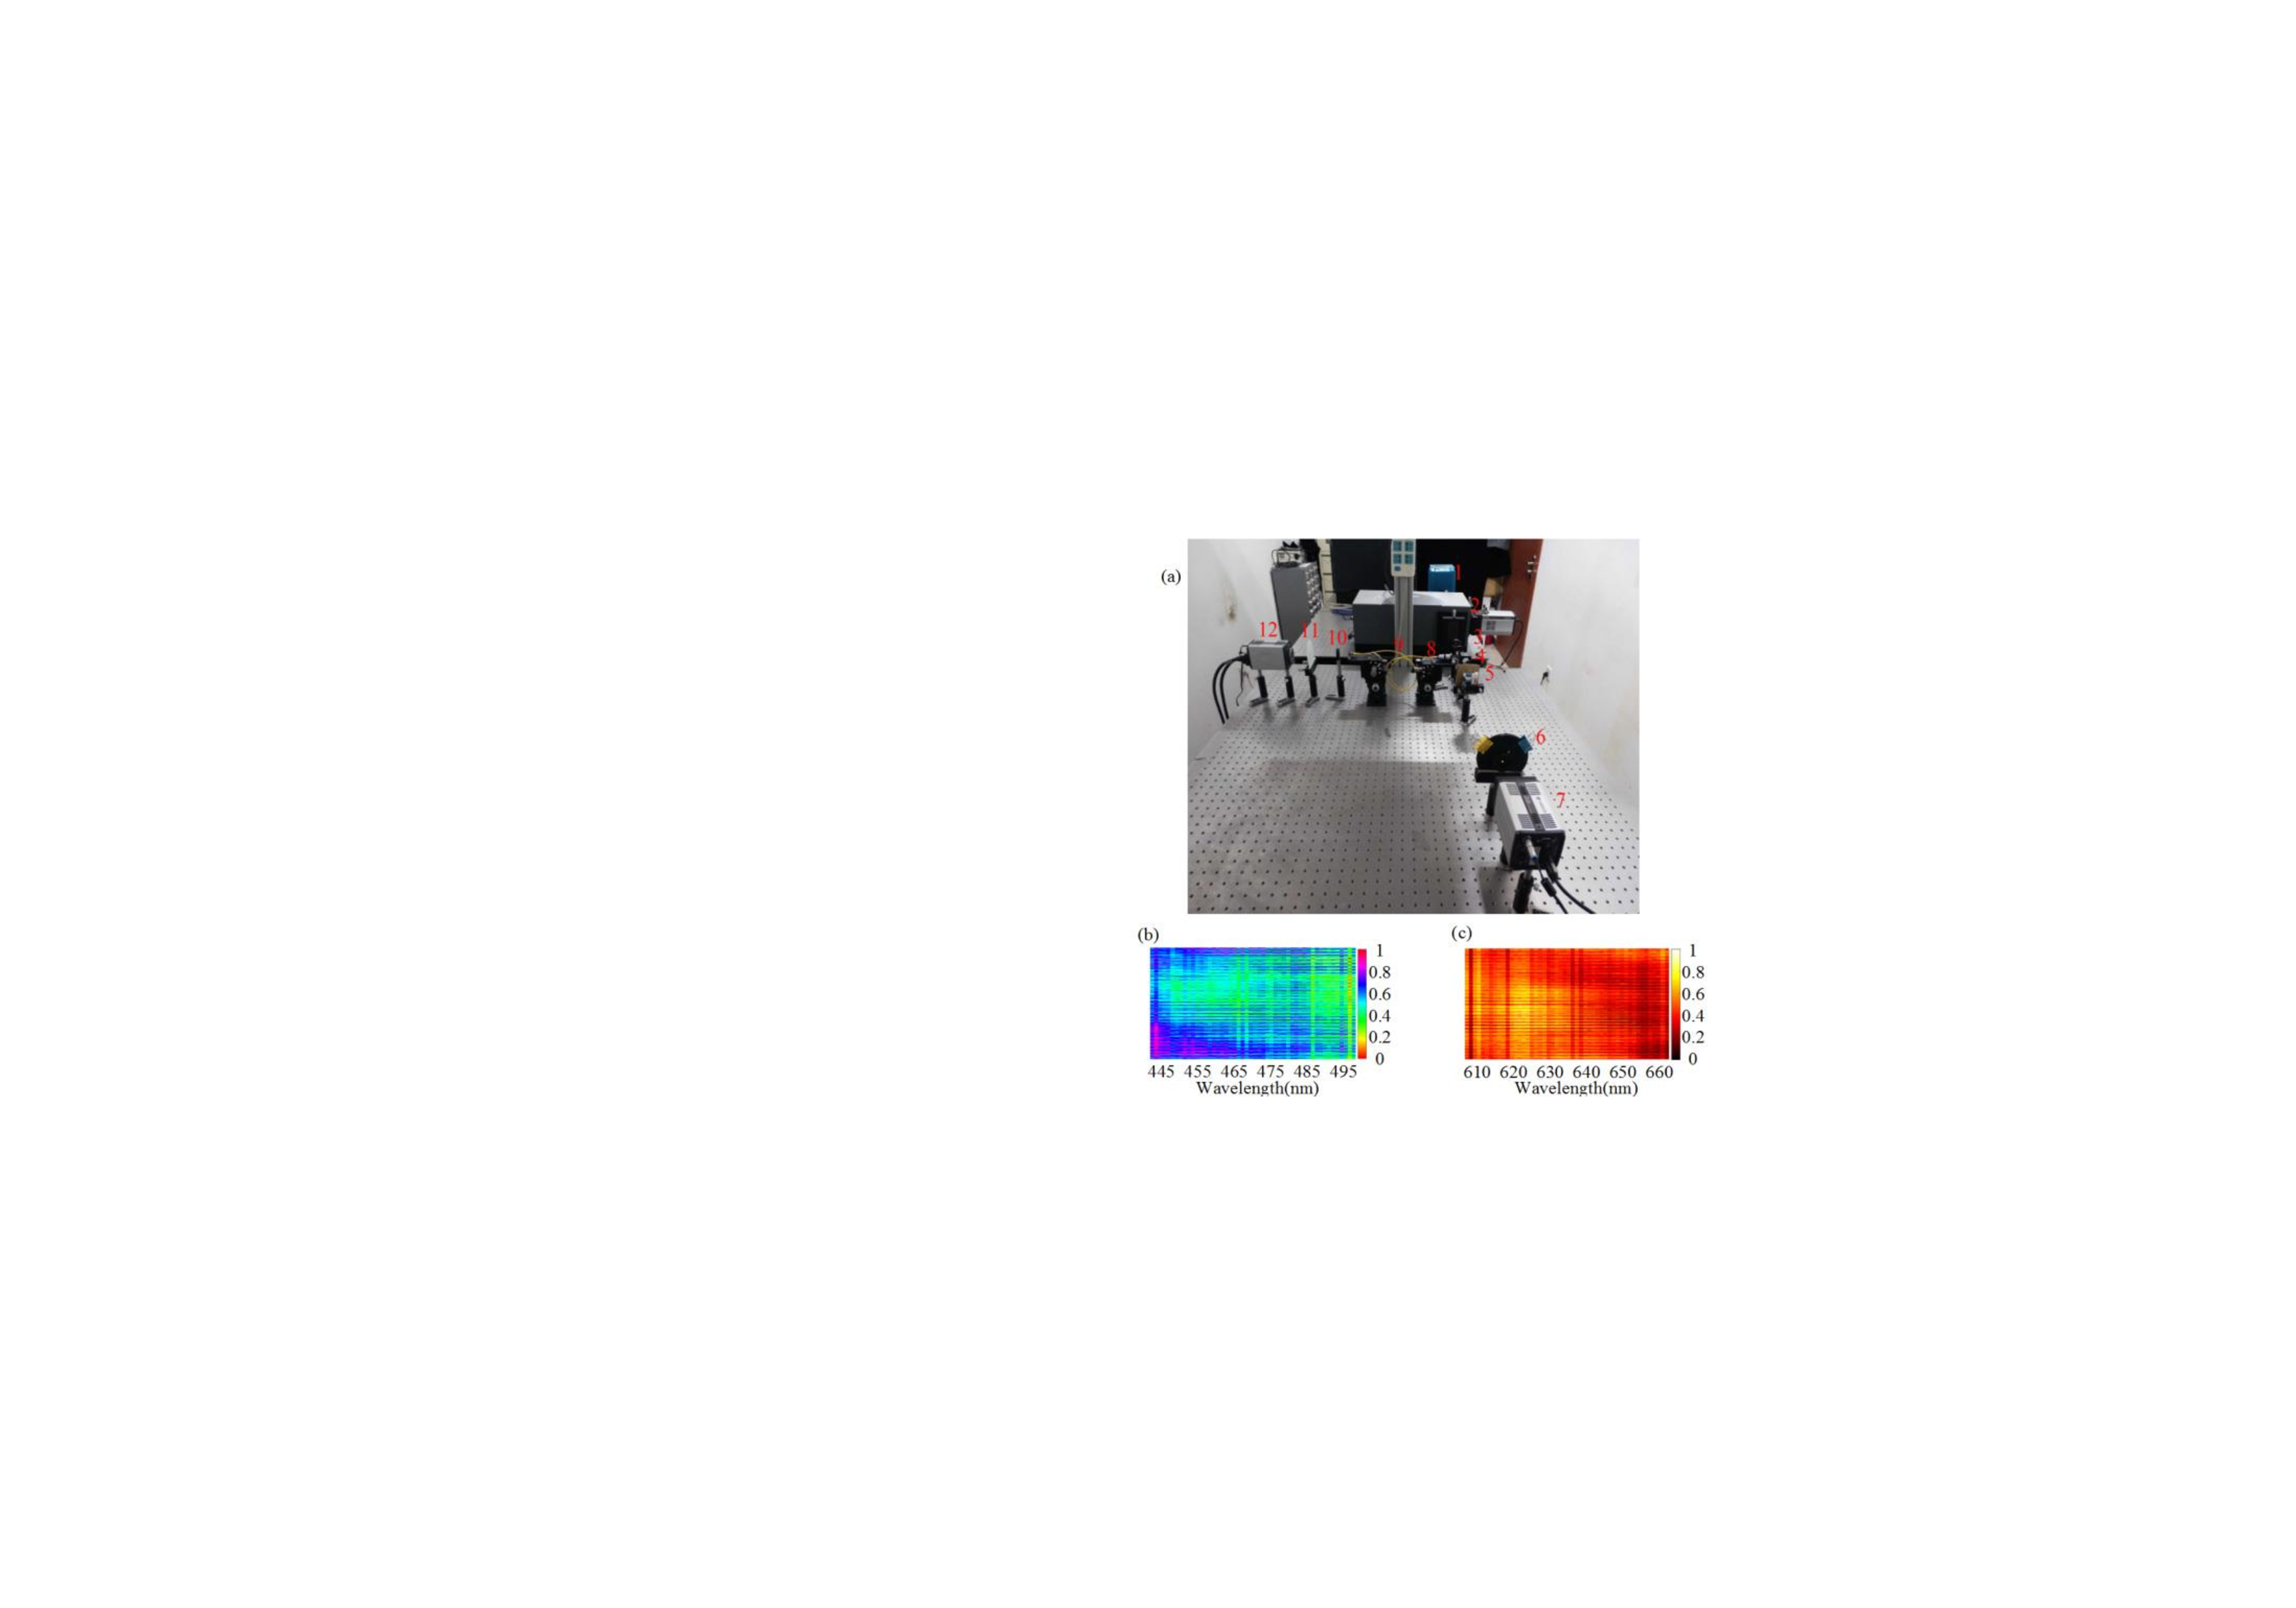
\includegraphics[scale=0.70]{C3.fig8.experimental_setup.pdf}
	\caption{光谱成像实验装置图}
	\label{fig:3.8}
\end{figure}

对于光谱标臂来说,我们利用物镜1和单模光纤对目标所发出的光进行收集,使用透镜对透过光纤后的光进行准直。这样的结构能够保证在我们的实验过程中,只需要对光谱臂进行的单次的光谱矩阵标定。
当完成光谱预标定后,我们采用了不同的目标对我们的系统进行测试,实验结果如图\ref{fig:3.9}所示。图\ref{fig:3.9}(a)和\ref{fig:3.9}(b)为分别利用单色光源照明时光谱信息恢复和目标空间信息重建结果,值得强调的是,此时我们使用的照明波长为已标定的光源波长。
我们的系统是否对未标定的连续光谱光源是否有效?们将在接下来部分进行详细分析。

\begin{figure}[htp]
	\centering
	
\includegraphics[scale=0.80]{C3.fig9.experimental_setup.pdf}
	\caption{光谱成像实验结果图}
	\label{fig:3.9}
\end{figure}

\subsection{光谱重建分析}
对于我们的照明光源可以分为两种:窄带光源和宽谱光源。为了验证光谱重建的有效性,首先我们利用已标定的光谱波段作为照明光源,进行光谱重建的有效性验证。光谱标定矩阵如图\ref{fig:3.8}b所示,在$445 \sim 495nm$光谱范围内,利用可调光源分别产生单色光源对目标进行照明,波长分别为:$459nm$、$466mn$、$473nm$和$481nm$,并对其光谱信号进行重建,重建结果如所示\ref{fig:3.10}(a)。从图\ref{fig:3.10}(a)可以看出,在于单色光源照明时,我们能够有效的重建照明的光源的光谱信息。同理,在$610 \sim 660nm$光谱范围内,进行了相同的实验,实验结果如图\ref{fig:3.10}(b)所示。

\begin{figure}[htp]
	\centering
	
\includegraphics[scale=0.70]{C3.fig11.experimental_setup}
	\caption{光谱重建结果}
	\label{fig:3.10}
\end{figure}

此后,我们采用更多标定的单色光源进行照明,并分别对光谱信号进行重建,实验结果如图\ref{fig:3.11}所示。从图\ref{fig:3.11}可以看出,重建信号与输入信号的光谱信号具有一致性。当连续光谱光源照明时,是否能够有效地重建光谱信号?因为已在仿真部分进行验证,所以此处我么将直接进行实验验证。首先采用LED光源作为照明光源,其中心波长和带宽分别为:$470nm$和$14nm$,其光谱重建结果和空间信息重建结果如图\ref{fig:3.12}(a)所示。为了进一步验证宽谱照明的有效性,利用红光LED进行照明,其中心波长和带宽分别为:$625nm$和$14nm$,对应的实验结果如图\ref{fig:3.12}(b)所示。至此,我们分别对窄谱和连续光谱照明时的光谱重建有效性进行了仿真验证和实验验证。

对比图\ref{fig:3.9}和\ref{fig:3.12},可以明显看出窄谱光源照明时,图像重建的效果优于宽谱光照明时的图像重建效果。我们将在接下来部分进行分析。

\begin{figure}[htp]
	\centering
	
\includegraphics[scale=0.70]{C3.fig10.experimental_setup}
	\caption{光谱重建结果}
	\label{fig:3.11}
\end{figure}
\begin{figure}[htp]
	\centering
	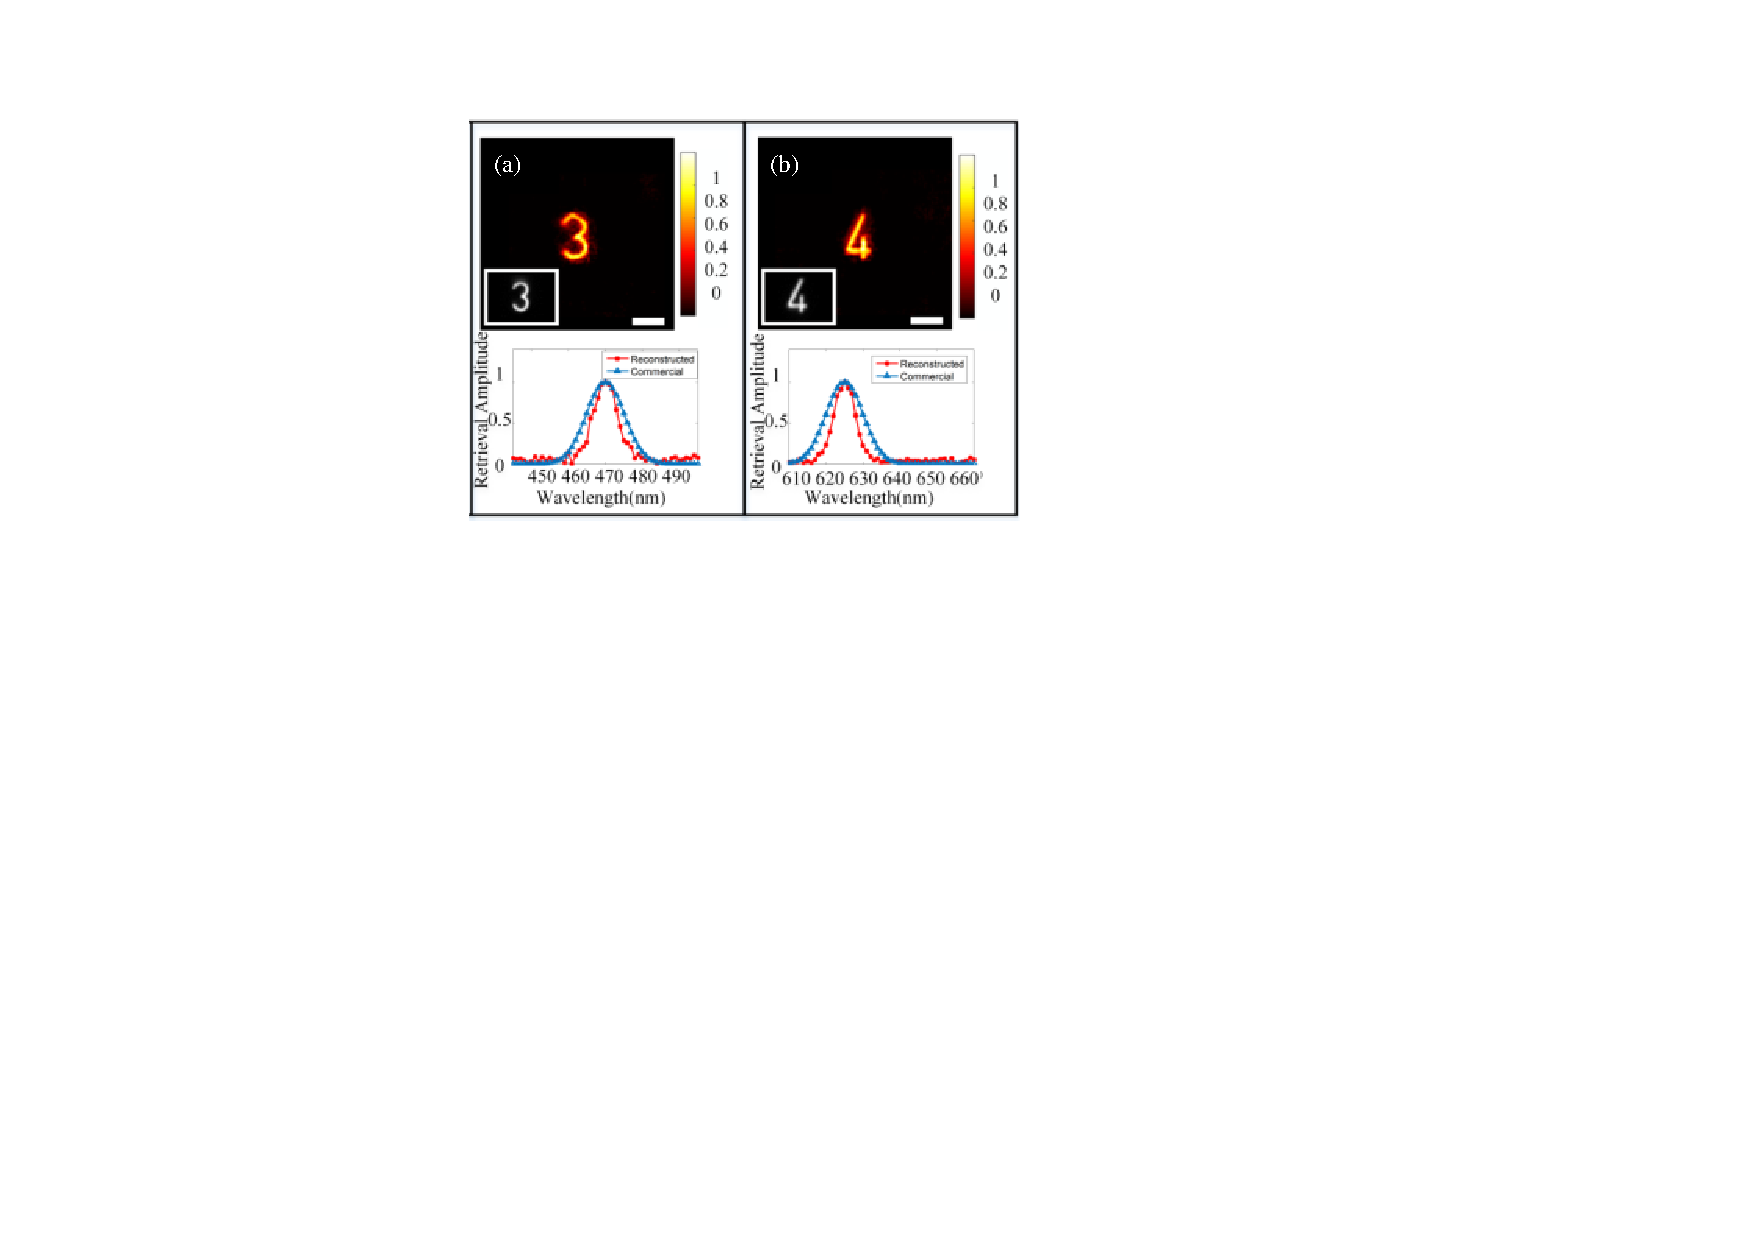
\includegraphics[scale=0.70]{C3.fig12.experimental_setup}
	\caption{宽谱照明时实验结果}
	\label{fig:3.12}
\end{figure}

\subsection{散斑相关成像分析}
为了分析不同带宽光源照明时,对于散斑相关成像的效果影响,我们分别利用窄谱和宽谱光源进行照明,并分别利用散斑相关成像技术进行图像恢复,实验结果如图\ref{fig:3.13}所示。实验中采用了FWFM分别为:$1nm$和$16nm$的照明光源。
\begin{figure}[htp]
	\centering
	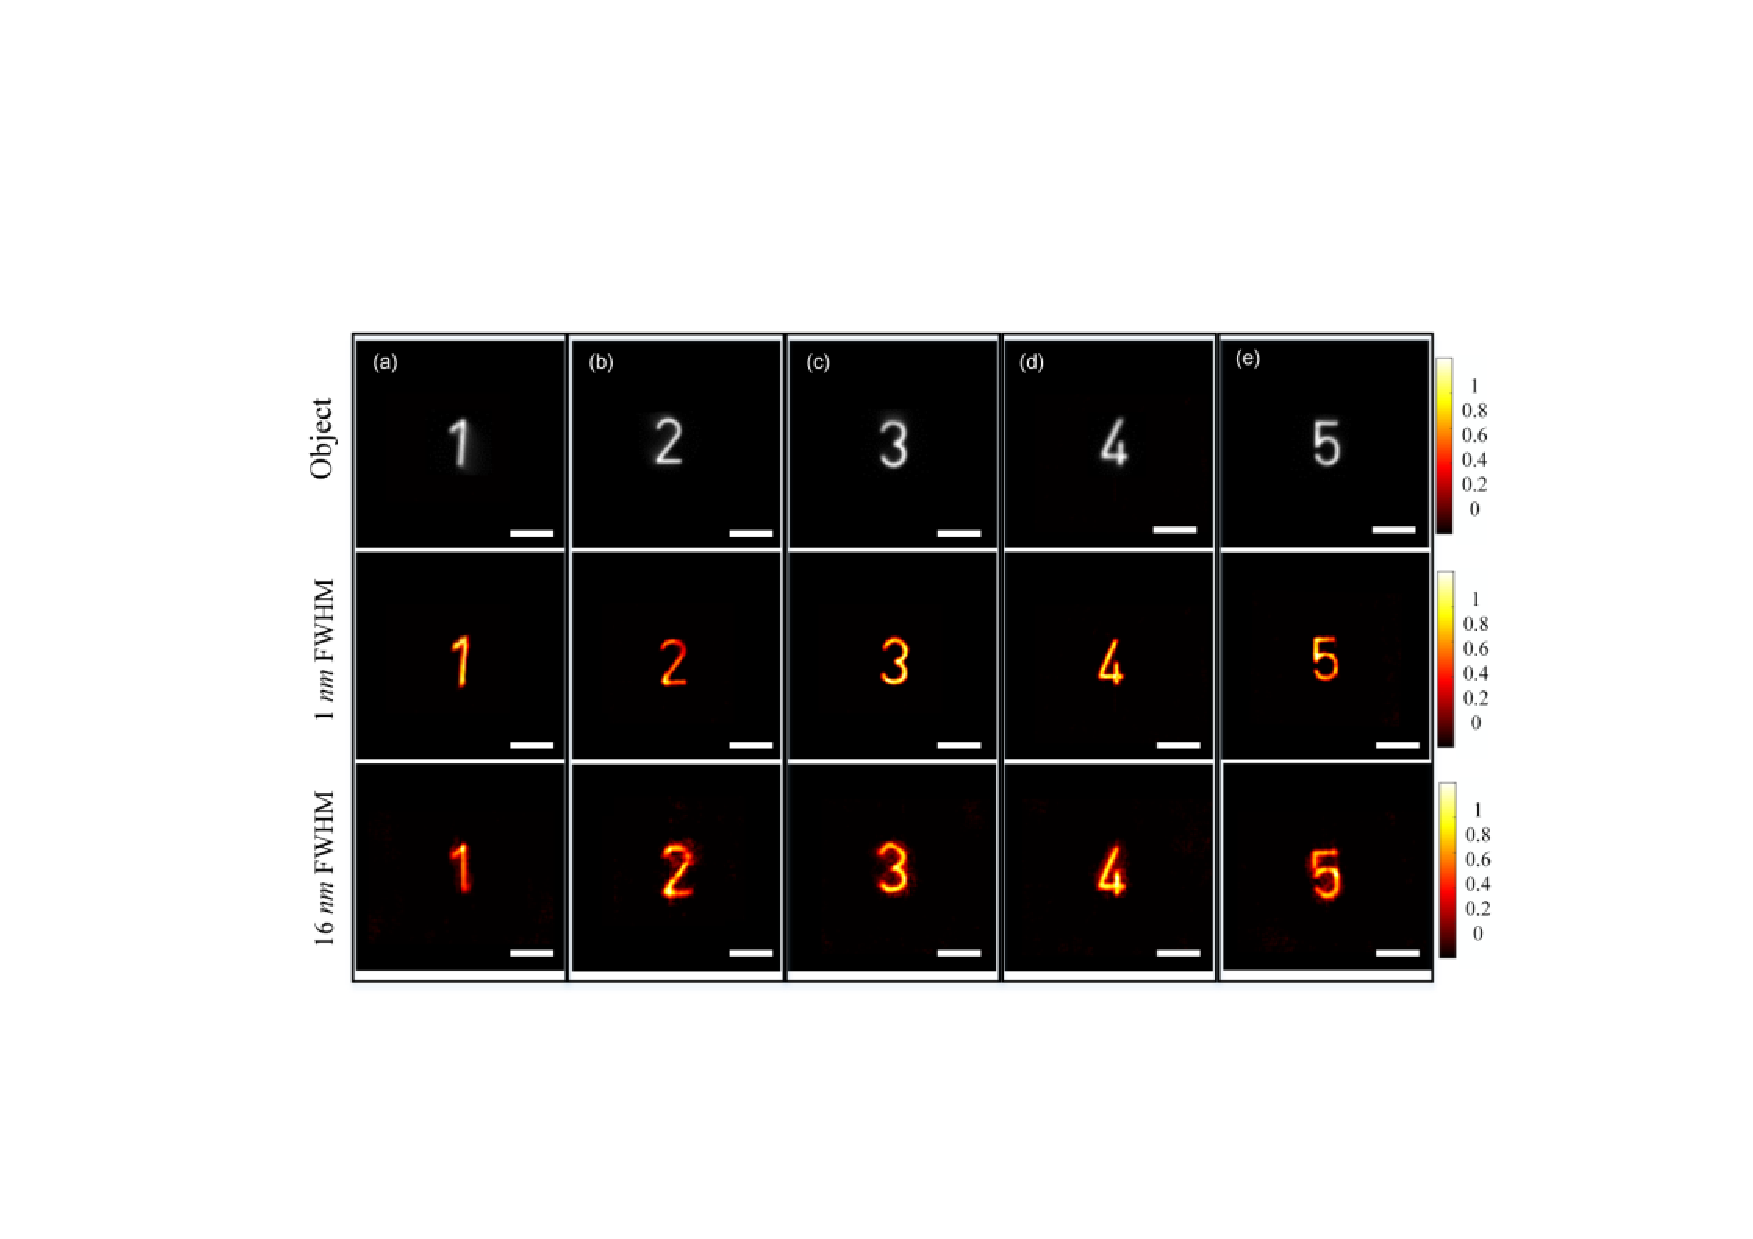
\includegraphics[scale=0.70]{C3.fig14.spectral_retrieval_model}
	\caption{宽谱照明时实验结果}
	\label{fig:3.13}
\end{figure}
从图\ref{fig:3.13}可以看出,窄谱光源照明时所对应的图像重建结果优于宽谱光源照明时的成像结果,造成此现象的的主要是由散斑的相关性变化引起的。理论上,当利用窄谱光源照明时,其散斑相关成像的理论模型如公式(\ref{eq:autocorelation_equation_1})所示。当使用宽谱光源照明时,散斑成像的理论模型为:

\begin{equation}
\begin{aligned}
    I \bigstar I  &= (O*S) \bigstar (O*S) \\
		              &=  (O \bigstar O)*\{\sum_{i=1}^{M} S_{\lambda_i} \bigstar S_{\lambda_i}+ \sum_{i=1}^{M}\sum_{i \ne j}^{M} S_{\lambda_i} \bigstar S_{\lambda_j})
\end{aligned}
\label{eq:autocorelation_wide}
\end{equation}
其中,$S_{\lambda_i}$为系统PSF,$\lambda_i$为照明光源波长。与公式(\ref{eq:autocorelation_equation_1})相比,公式(\ref{eq:autocorelation_wide})拥有额外项$\sum_{i=1}^{M}\sum_{i \ne j}^{M} S_{\lambda_i} \bigstar S_{\lambda_j}$。当使用窄谱光源照明时,$\sum_{i=1}^{M}\sum_{i \ne j}^{M} S_{\lambda_i} \bigstar S_{\lambda_j}$的值远远小于$\sum_{i=1}^{M} S_{\lambda_i} \bigstar S_{\lambda_i}$项,可忽略不计,在最终的相位恢复过程中影响可以忽略。当使用宽谱光源照明时,$\sum_{i=1}^{M}\sum_{i \ne j}^{M} S_{\lambda_i} \bigstar S_{\lambda_j}$的值随之增加,导致所恢复目标的傅里叶振幅信息中具有较多噪声,进而致使最终的重建效果变差。从图\ref{fig:3.13}可以看出,随着照明光源的带宽增加,重建结果变得模糊。实验结果与理论分析相一致。
\section{光谱传输矩阵方法的扩展}
在\ref{光谱传输矩阵章节}节中,我们对光谱传输矩阵的基本原理进行了阐述。此处的光谱传输矩阵本质上为强度光谱传输矩阵。我们能够利用此光谱传输矩阵,从散斑图像中恢复光谱信息。此光谱传输矩阵的核心思想为:建立了光谱信息与散斑图案的一一对应关系。是否能够受到此思想的启发,建立空间信息与光谱信息的一一对应关系,进而实现目标空间信息的重建?答案是:YES。当光通过折射率非均匀介质时,如:毛玻璃、纸张、生物组织等,会引起散射效应,出射光场变得紊乱而随机,形成一系列散斑。传统的光学成像方法在散射作用的影响下无法有效地获得目标信息,因此研究透过散射介质的新型成像方法具有重要的意义。迄今为止,利用光学散射特性成像技术已经展开了大量研究,例如,已提出了波前调制、光学相干层析、超快激光飞行时间成像法、散射矩阵测量、散斑相关等方法。2007年,I.M. Vellekoop等人首次提出了波前调制技术对入射光波前进行调制,实现了透过散射介质聚焦与成像。 但波前调制技术有很大的局限性:首先,波前调制技术需要复杂的反馈调制过程,才能实现明显的聚焦效果;其次,波前调制技术属于主动式成像,无法用于被动式成像系统。 2012年,J. Bertolotti等提出了一种非侵入式散射成像方法。该方法利用OME,通过计算强度散斑的自相关并结合相位恢复算法实现了透过散射介质成像。2014年,O. Katz等提出了一种基于OME的单帧散斑自相关的散射成像方法,该方法不仅保持了原有方法非侵入式成像的特点,而且具有极高的时间分辨率,在活体生物样本成像领域有巨大潜力. 同时,A. K. Singh等利用无透镜傅立叶全息成像技术,通过统计平均的方式抑制散斑实现了透过散射介质成像。 2016年,E. Edrei等提出了基于去卷积的透过散射介质的超分辨率显微成像,以系统PSF为先验知识,通过去卷积的方法实现透过散射介质成像. 综上所述,目前已有的透过散射介质成像方法受到以下限制:(\romannum{1}) 需要接收完整的散斑信号;(\romannum{2}) 需要窄谱光源作为照明光源. 因此,如何突破这些限制对于透过散射介质成像的发展具有重要意义。

此处,我们提出基于空间-光谱传输矩阵(Spatial-Spectral Transmission Matrix,SSTM)的散射成像方法,结合非线性优化算法,有效地利用散射介质的随机色散特性实现了透过散射介质成像。与传统散射成像方法相比,基于SSTM的散射成像方法无需接收散斑,并且以宽谱光源作为照明光源,实现了透过散射介质成像。其基本思路是点源目标经过散射介质后在像面形成散斑,利用光谱仪接收像面上固定位置的光谱信号,将不同位置点源目标对应的光谱信号组成光谱传输矩阵,最后利用目标重建算法实现透过散射介质成像。该方法的核心思想为:利用散射的介质的光谱多样性和空间多样性,建立空间信号与光谱信号的对应关系,结合非线性优化算法,进而实现了透过散射介质的成像。
\subsection{基本原理}

散射介质作为一个随机的二维光谱色散元件,当入射光透过散射介质时会受到散射作用的影响,在像面形成散斑. 对于像面上的散斑分布而言,不同空间位置点源目标对应的散斑分布不同,其光谱信息也存在差异。当照明光源一定时,相机面所接收的散斑分布可以由公式(\ref{eq:wavelength_diversity})可知。相机面所接收到强度与各个点源目标位置之间的关系,其所接收到强度信号可以表示为:
\begin{equation}
    I(r_{c},\lambda) = |E(r_{c},\lambda)|^2 = |A\iint E(r_{o},\lambda)e^{\frac{ik}{2d}(r_{s}-r_{o})^{2}}Pup.(r_{s},\lambda)T(r_{s},\lambda)e^{\frac{ik}{2S_{o}}(r_{c}-r_{s})^{2}}\mathrm{d}{r_{o}}\mathrm{d}{r_{s}}|^2
\label{eq:wavelength_dependent},
\end{equation}
为了方便分析点源目标与相面所接收到散斑信号分布关系,所以将公式(\ref{eq:wavelength_dependent})简化为:
\begin{equation}
    I(r_{c},\lambda) = A^2|\iint E(r_{o},\lambda) \beta (r_o,r_s)\mathrm{d}{r_{o}}\mathrm{d}{r_{s}}|^2
\label{eq:wavelength_dependent_1}
\end{equation}
其中,$\beta(r_o,r_s,\lambda) = e^{\frac{ik}{2d}(r_{s}-r_{o})^{2}}Pup.(r_{s},\lambda)T(r_{s},\lambda)e^{\frac{ik}{2S_{o}}(r_{c}-r_{s})^{2}}$,$k=2\pi/\lambda$。
\begin{figure}[htp]
	\centering
	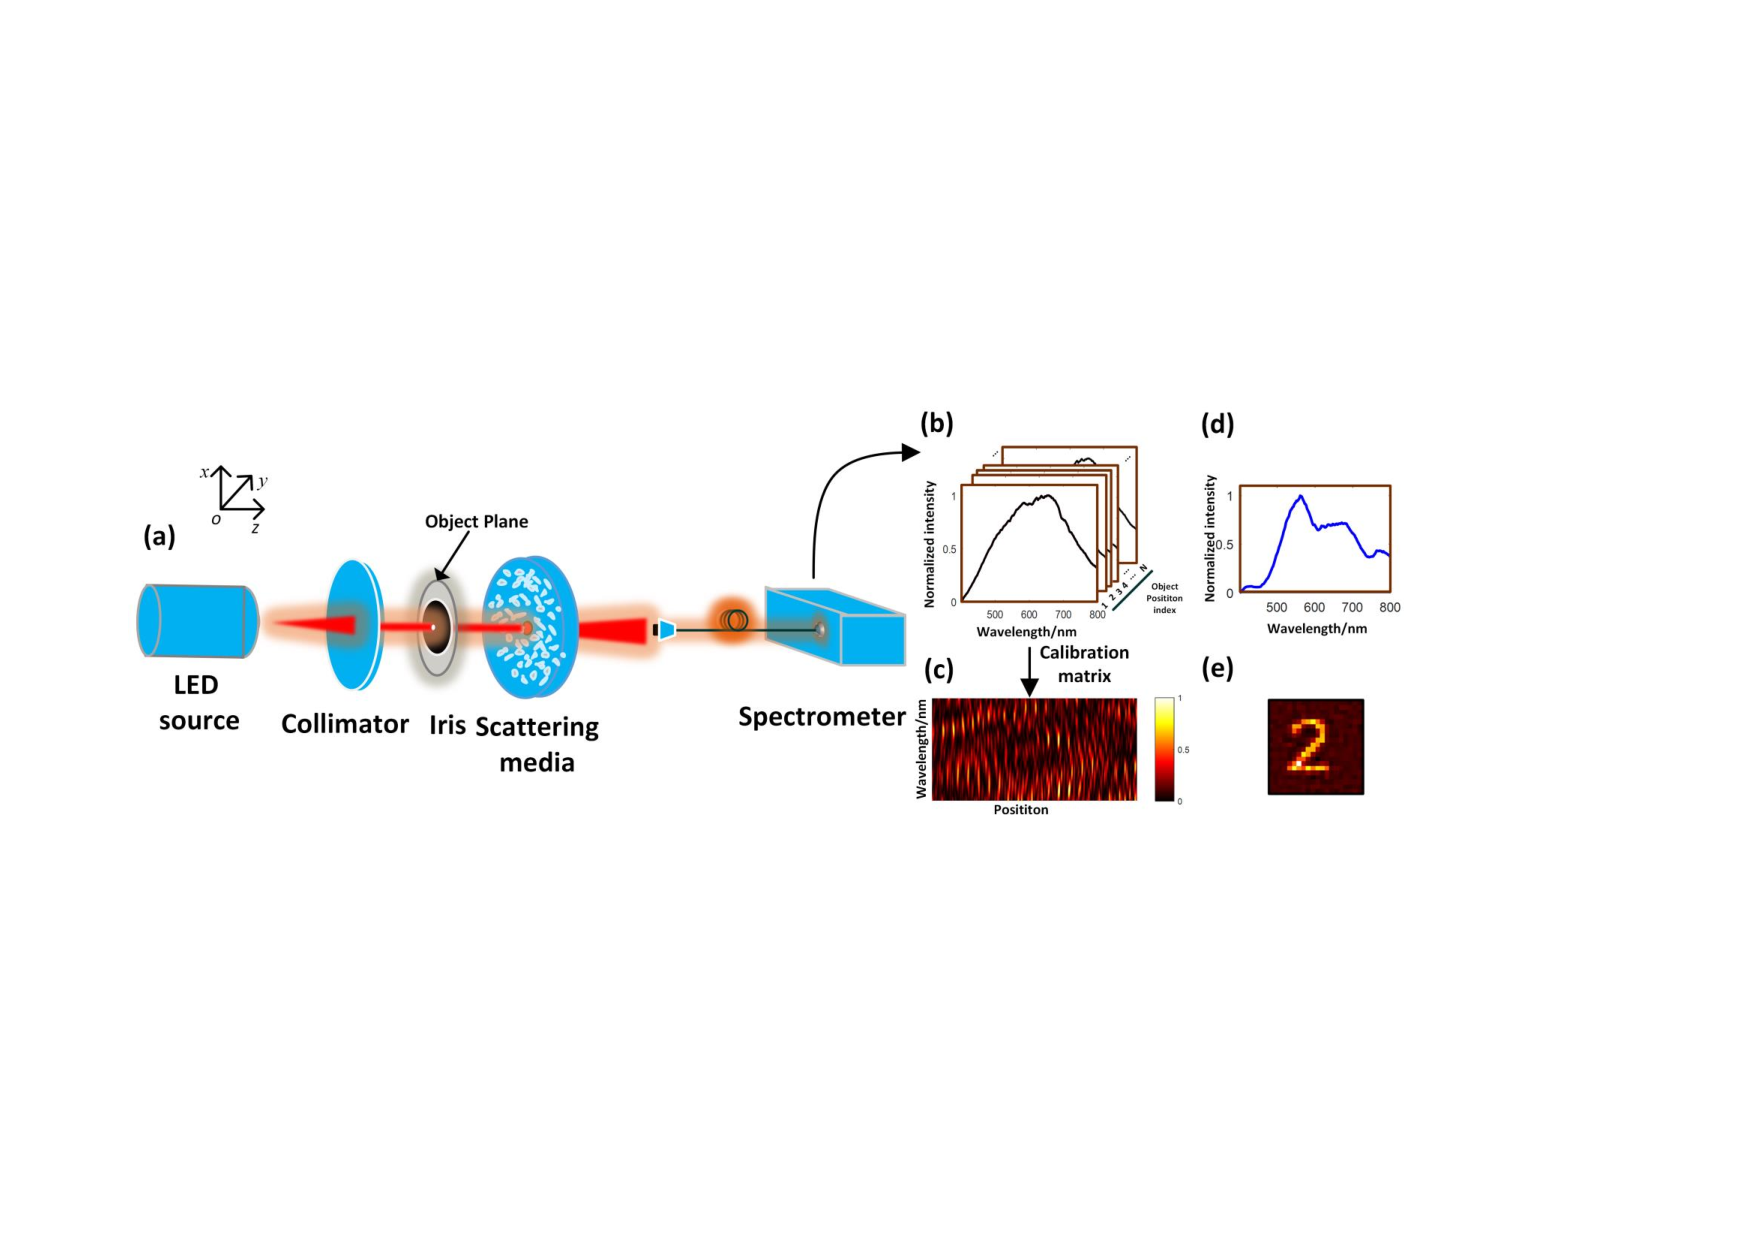
\includegraphics[scale=0.70]{C3.fig15.spectral_retrieval_model}
	\caption{基于SSTM的透过散射介质成像系统示意图}
	\label{fig:3.15}
\end{figure}
因此,当在相机面选定感兴趣区域时,该区域所接收到的光谱信号可以表示为:
\begin{equation}
    \mathsf{S}_{r_{c}}(\lambda) = \int I(r_{c},\lambda) \mathrm{d}{r_{c}}
\label{eq:wavelength_dependent_2}
\end{equation}

通过分析式(\ref{eq:wavelength_dependent})-(\ref{eq:wavelength_dependent_2})可知,像面的散斑图样分布的细节依赖于散射介质的所引起的相位变化和照明光的波,也取决于点源目标的位置。同时散射介质具有波长多样性和角度多样性,所以当系统其它参数一定时,点源目标的位置发生改变,散斑的图样也会发生变化。同理,当照明光源的位置发生变化时,相机感兴趣区域所接收的接收到的光谱信号也会随之改变。所以利用源目标的位置改变带来的光谱多样性,结合SSTM实现透过散射介质成像。
\subsection{SSTM标定原理}
图\ref{fig:3.15}为基于SSTM的透过散射介质成像系统示意图,系统主要包括:宽谱LED光源、准直系统、光阑、散射介质和光纤光谱仪。光源发出的光经过准直器准直后,照射在光阑上形成点源目标,点源目标的光透过散射介质,最终在像面上形成散斑,光谱仪用来接收像面上固定的位置的光谱信号。

SSTM标定方法如下:首先,经准直后的白光LED光源(具有一定光谱带宽)经过光阑(光阑空间位置为$r_1$,如图\ref{fig:3.16}(a)所示),入射到散射介质表面,在介质后方形成随机的散斑场,利用光谱仪在固定位置接收光谱信号$\mathsf{S}_{r_{1}}$;其次,将光阑位置移动至$r_2$,光谱仪保持位置不变接收相应的光谱信号$\mathsf{S}_{r_{2}}$;依次移动光阑位置对物面进行扫描,光阑的移动路径如图\ref{fig:3.16}(a)中白色箭头所示,分别记录不同物空间位置对应的光谱信号$\mathsf{S}_{r}$;最后,将不同的物空间位置对应的$\mathsf{S}_{r}$合成后的SSTM如图\ref{fig:3.16}(b)所示,即完成SSTM标定。SSTM $\mathbb{S}$ 可表示为:
\begin{equation}
    \mathbb{S} = [\mathsf{S}_{r_{1}},\mathsf{S}_{r_{2}},\cdots,\mathsf{S}_{r_{n}},\mathsf{S}_{r_{n+1}}\cdots]
\label{eq:wavelength_dependent_3}
\end{equation}

\begin{figure}[htp]
	\centering
	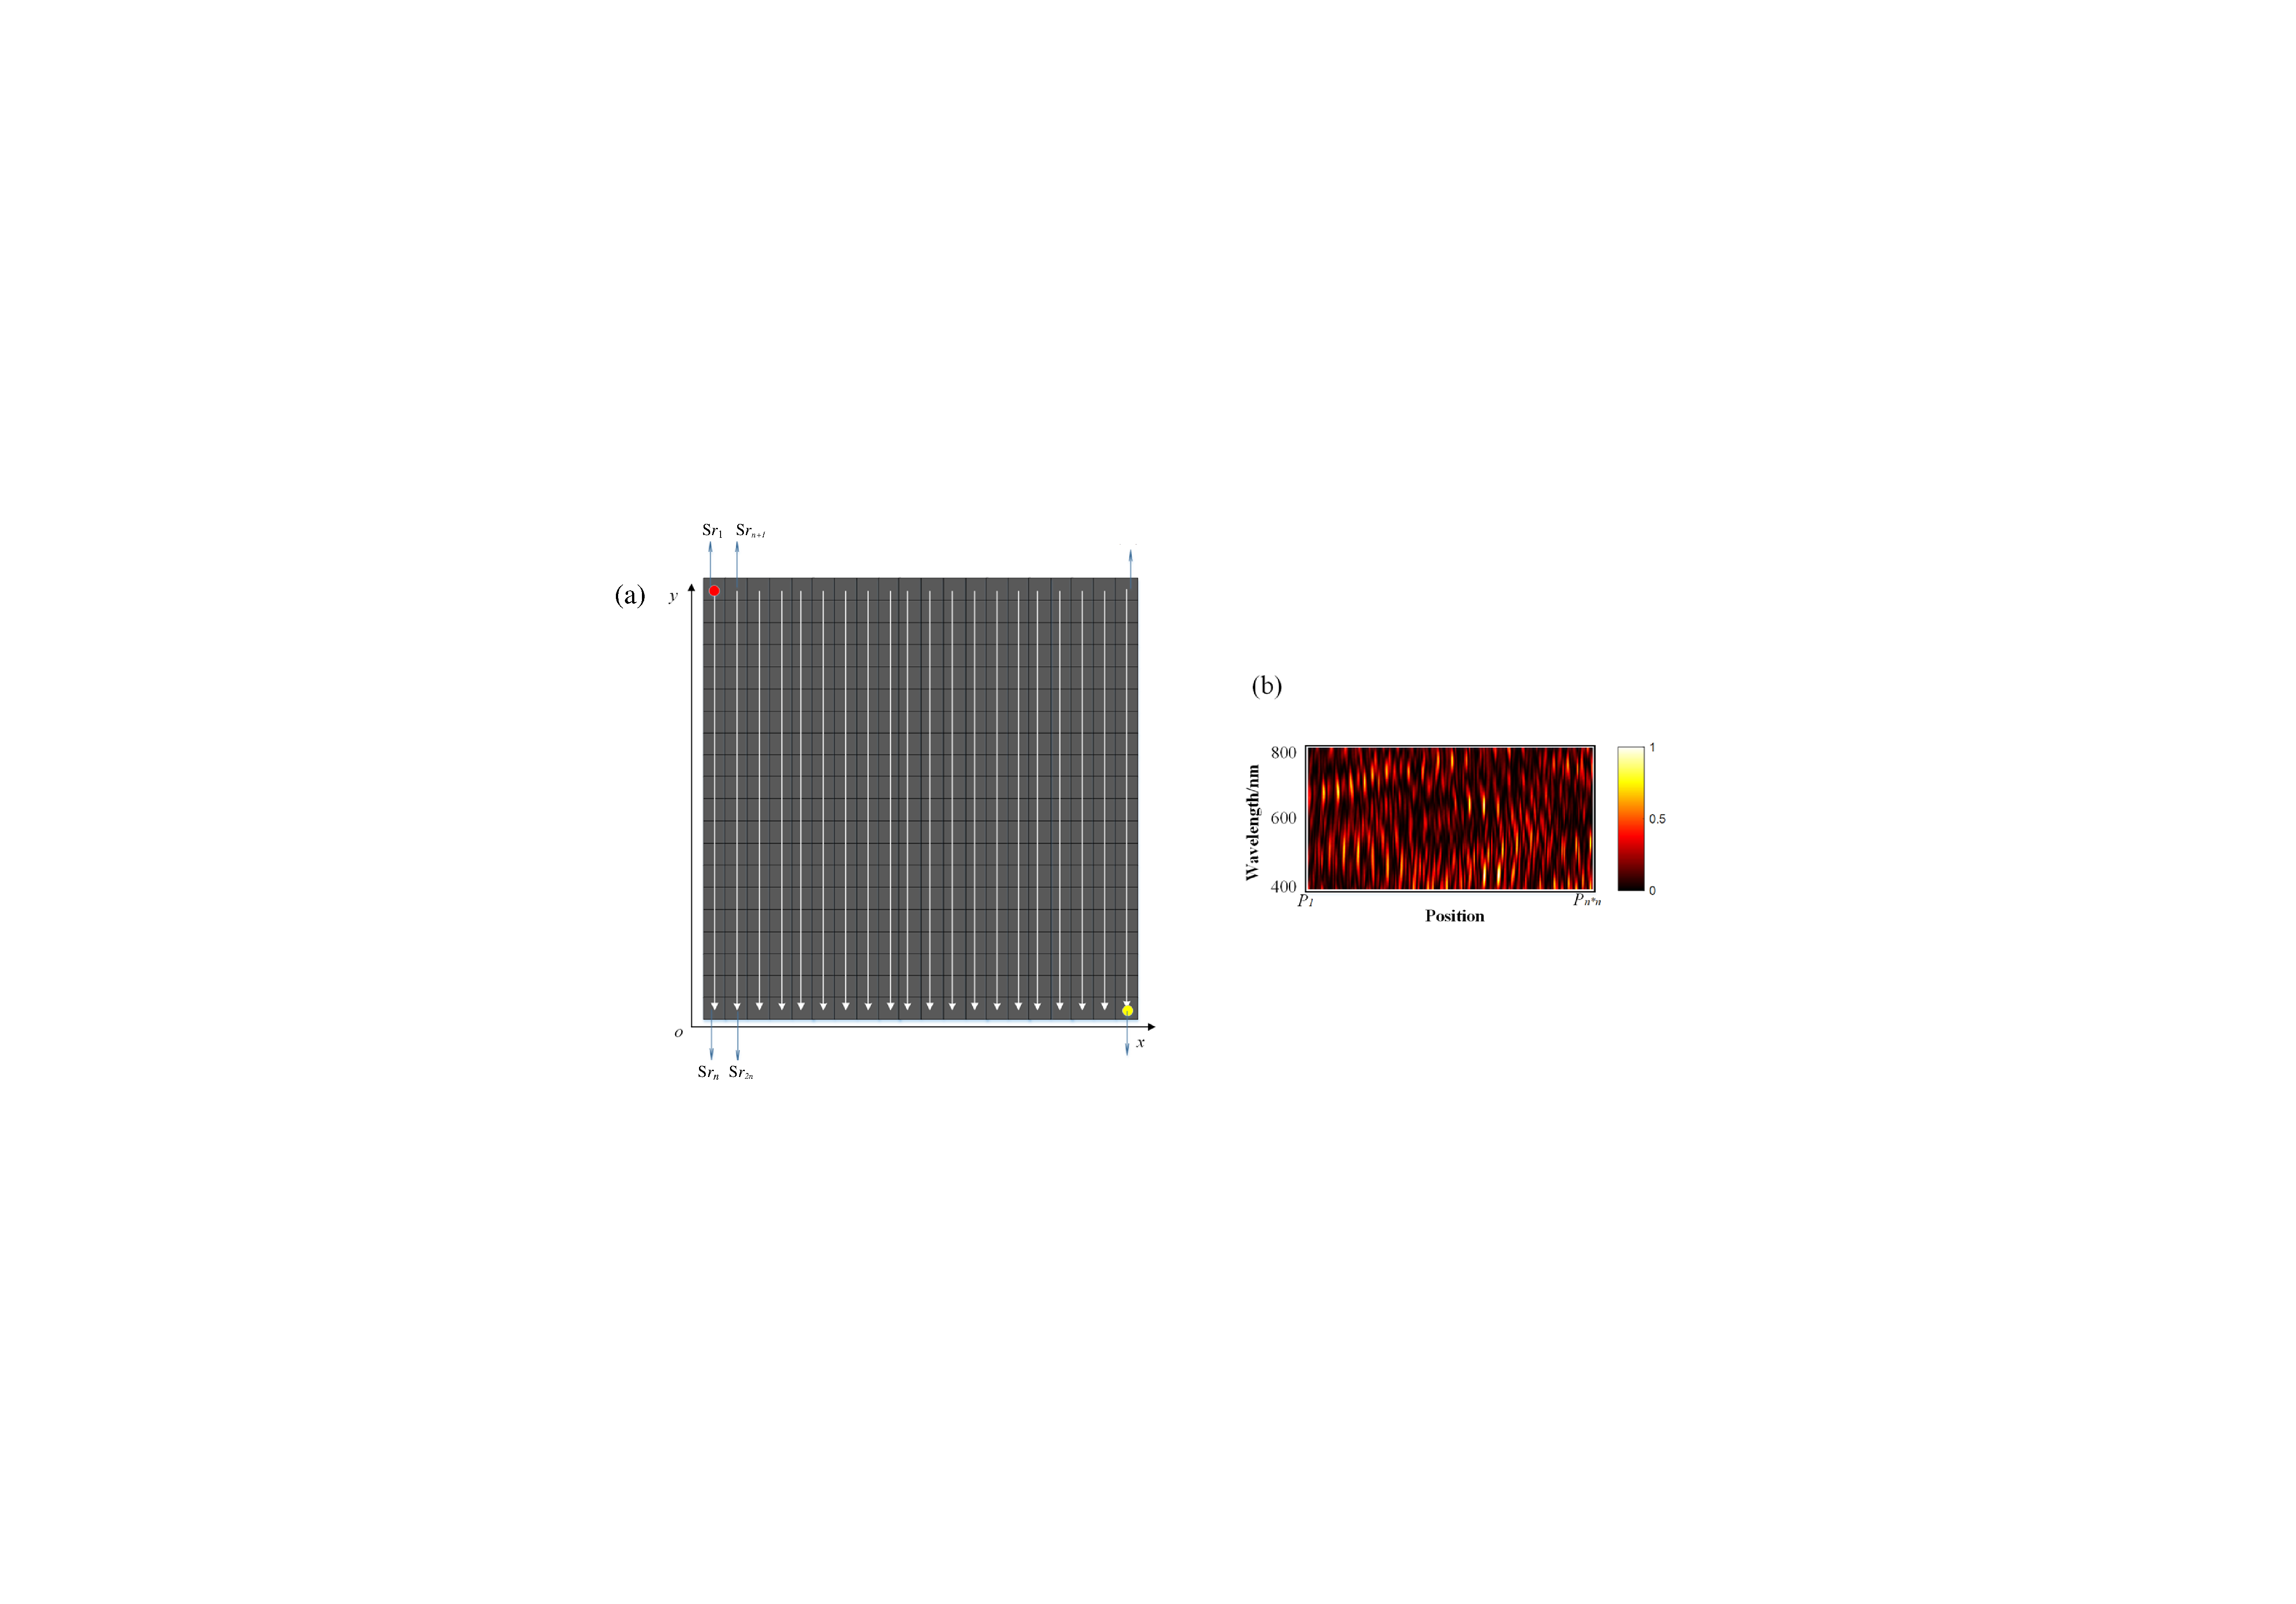
\includegraphics[scale=0.35]{C3.fig16.spectral_retrieval_model}
	\caption{SSTM标定示意图}
	\label{fig:3.16}
\end{figure}

\subsection{目标重建算法}
基于光谱传输矩阵的透过散射介质成像模型可以表示为:

\begin{equation}
    \mathsf{S_{\textit{measured}}} =\mathbb{S}O
\label{eq:wavelength_dependent_4}
\end{equation}
其中:$\mathsf{S_{\textit{measured}}}$ 为光谱仪所接收的带重建目标产生的光谱信号;$\mathbb{S}$为光谱传输矩阵;$O$为待重建目标信号。

从计算角度考虑,对SSTM矩阵$\mathbb{S}$直接求逆,便可以重建出目标信号,即 $ O = \mathbb{S}^{-1} \mathsf{S_{\textit{measured}}}$,但在数学上,直接对$\mathbb{S}$求逆矩阵属于病态问题 (当矩阵的行和列不相等时)。传统的方法是采用SVD奇异值分解(Singular Value Decomposition,SVD)对矩阵求伪逆。因此,目标信号可以表示为:
\begin{equation}
  O = VD^{-1}U^{T}\mathsf{S_{\textit{measured}}}
\label{eq:wavelength_dependent_5}
\end{equation}
其中,上标$T$代表矩阵转置;$VD^{-1}U^{T}$是$\mathbb{S}$的SVD分解。

在实际实验中,噪声无法避免。如何有效地抑制噪声,将对该方法的使用有着重要的意义。我们在矩阵求逆算法的基础上,结合模拟退火算法,提出了一种混合型的非线性优化算法。在此混合型非线性优化算法中,将公式(\ref{eq:wavelength_dependent_5})所表示的成像模型转化为能量最小化模型,即:
\begin{equation}
  E = \| \mathsf{S_{\textit{measured}}}-\mathbb{S}O \|^2
\label{eq:wavelength_dependent_6}
\end{equation}
将矩阵求逆方法与模拟退火算法相结合,求解最优化$O$。在模拟退火算法的单次优化中,将$O$中的一个元素乘以随机数$\alpha (0.5≤a≤2.5)$,在此过程中将生成一个新的信号$O^{\prime}$。则能量改变可以表示为:
\begin{equation}
  \Delta E = \| \mathsf{S_{\textit{measured}}}-\mathbb{S}O \|^2-\| \mathsf{S_{\textit{measured}}}-\mathbb{S}O^{\prime} \|^2
\label{eq:wavelength_dependent_7}
\end{equation}
以$exp[ \Delta E / t_0]$ 概率接受$O$元素的更新(即:$O = O^{\prime}$),其中$t_0$为系统初始温度。在整个优化过程中,对$O$中的每个元素依次进行更新,并且系统温度$t$随着优化进行而减小。当系统温度较高时,模拟退火算法具有较高的概率去接受非准确的元素更新结果;当系统温度较低时,模拟退火算法具有较高的概率去接受更优化的元素更新结果 (注:当$\Delta E \ge 0 $时,$O$的元素更新结果全部被接受)。

于是,我们将矩阵求逆算法和所提出的混合型非线性优化算法进行对比,其结果如图\ref{fig:3.16}所示。其中,\ref{fig:3.17}a为矩阵求逆算法的重建结果;\ref{fig:3.17}b为混合型非线性优化算法的重建结果。为了定量化描述重建信号的误差,需要计算重建信号与已知信号之间的标准差$\mu$。

\begin{figure}[htp]
	\centering
	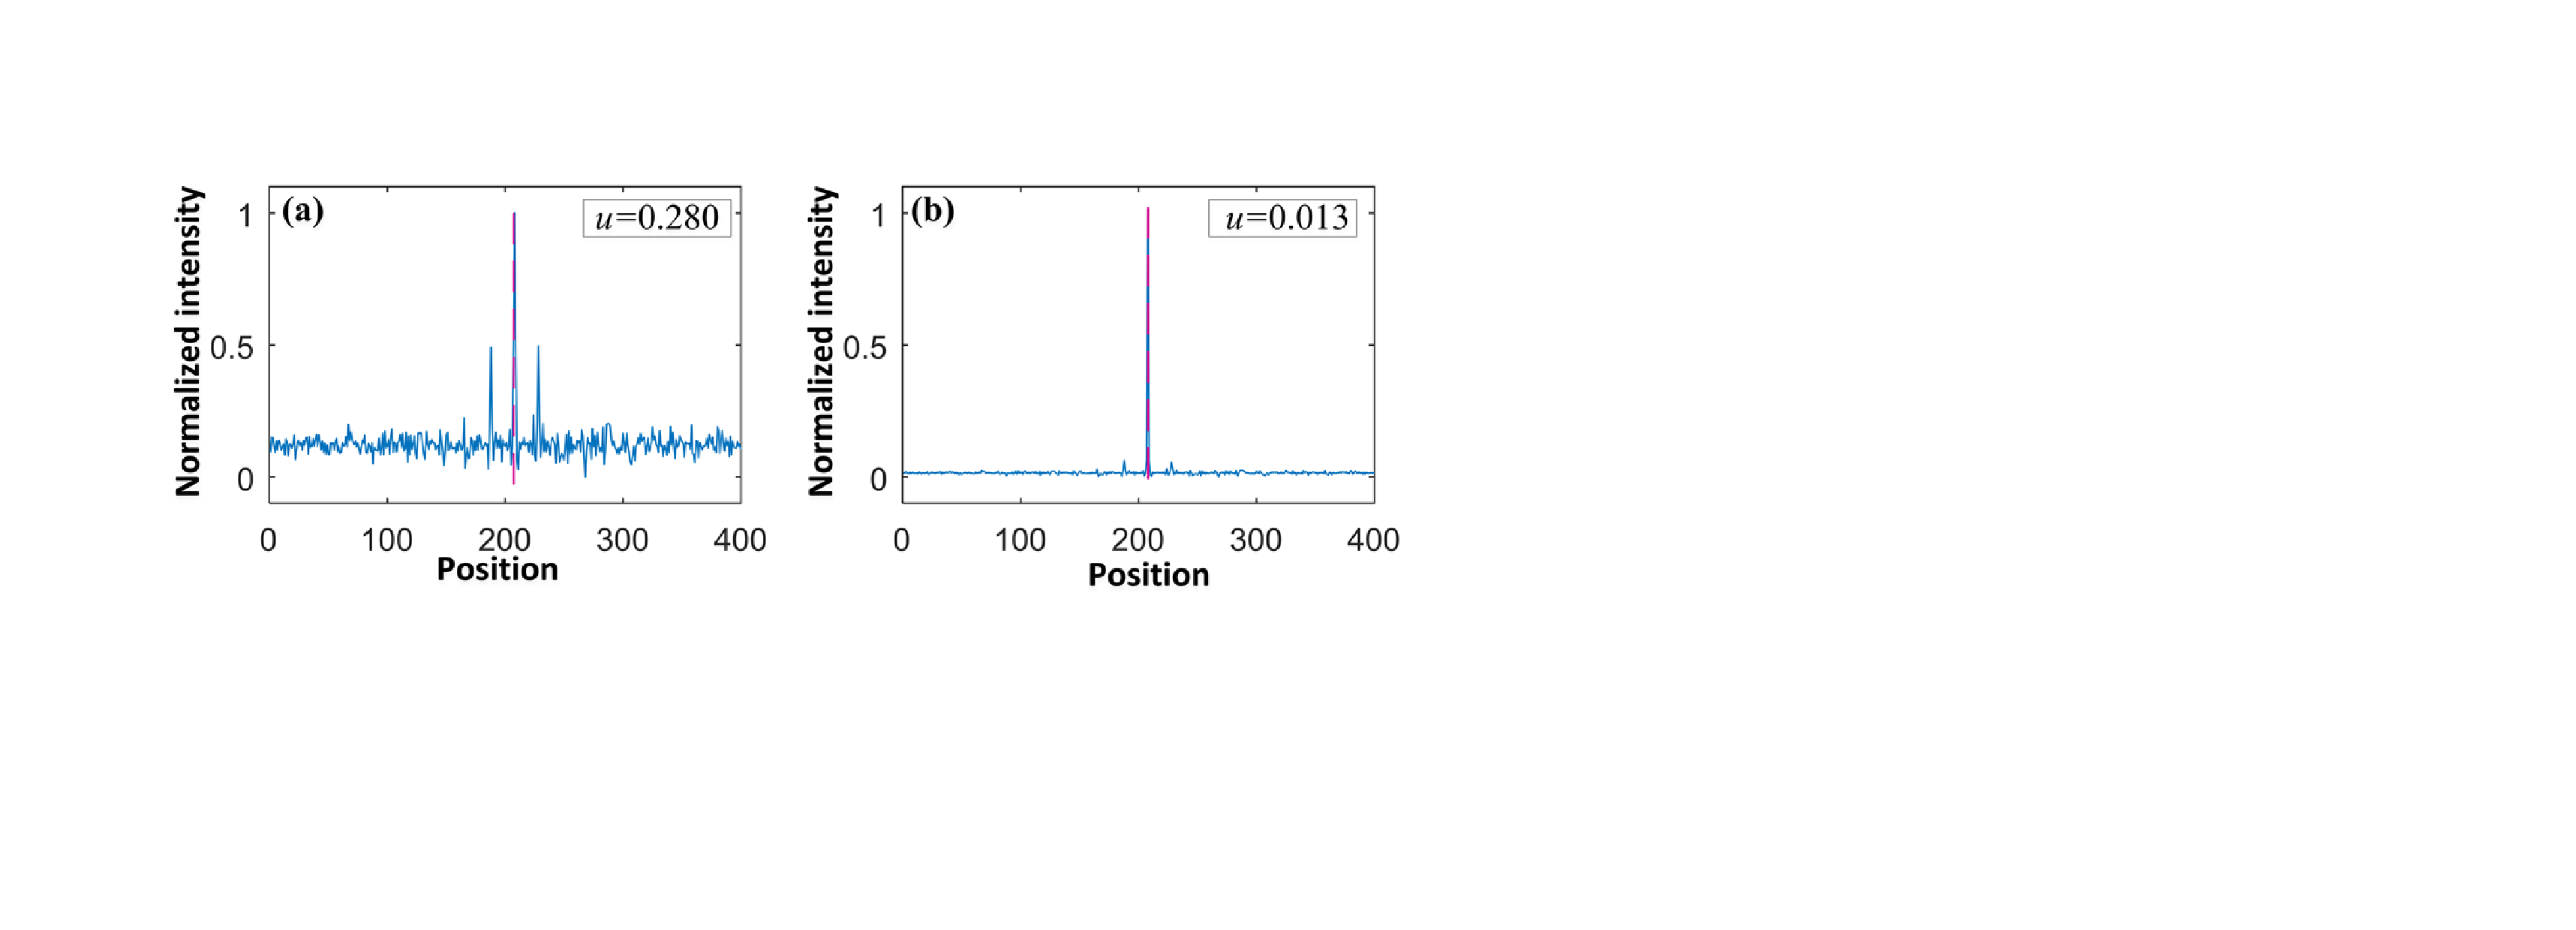
\includegraphics[scale=0.45]{C3.fig17.spectral_retrieval_model}
	\caption{不同算法的重建结果对比}
	\label{fig:3.17}
\end{figure}

由实验结果看出,利用矩阵求逆算法的重建信号与已知信号相对误差较大(标准差为0.280),无法有效抑制噪声,混合型非线性优化算法的的重建误差为0.013,有效地抑制了噪声并且减小了重建结果的误差。另外,传统的模拟退火算法一般需要几百次上千次优化才能寻找到最优化的结果。但是,我们所利用的混合型非线性优化算法利用矩阵求逆的方法给模拟退火算法提供初始猜测$O$,从而有效地减少了优化次数和抑制噪声,并且提高了重建信号的准确性。
\subsection{实验结果}
基于光谱传输矩阵的散射成像实验系统如图\ref{fig:3.15}所示。实验中,采用白光LED(Throlabs,QTH10,光谱的半高全宽FWHM:$230 nm$)作为光源,扩束准直器(Throlabs,GBE20-A)进行光束准直,散射介质(Thorlabs,DG10-220)置于光阑后 $200 mm$处和光谱仪(Throlabs,CCS200)置于散射介质后 $180 mm$处。因为本系统的空间分辨率约为$100 \mu m$,于是实验中选用的光阑孔径为$200 \mu m$。利用三维位移平台(Throlabs,MBT613D/M)将光阑位置按图\ref{fig:3.16}所示的标定方法实现SSTM标定,位移平台步进为$100 \mu m$,将物面$ 4\times 4 mm^2$ 的面积划分为$ 20\times 20$ 等大小网格。

当光谱传输矩阵标定完成后,首先以点源作为目标,验证基于SSTM的散射成像效果。实验结果如图\ref{fig:3.18}所示,图\ref{fig:3.18}a为原始目标、图\ref{fig:3.18}b为利用矩阵求逆所重建目标的结果和图\ref{fig:3.18}c为混合型非线性优化算法实现目标重建的结果。通过对比可以看出,混合型非线性优化算法对噪声的抑制效果明显优于传统的矩阵求逆算法。
\begin{figure}[htp]
	\centering
	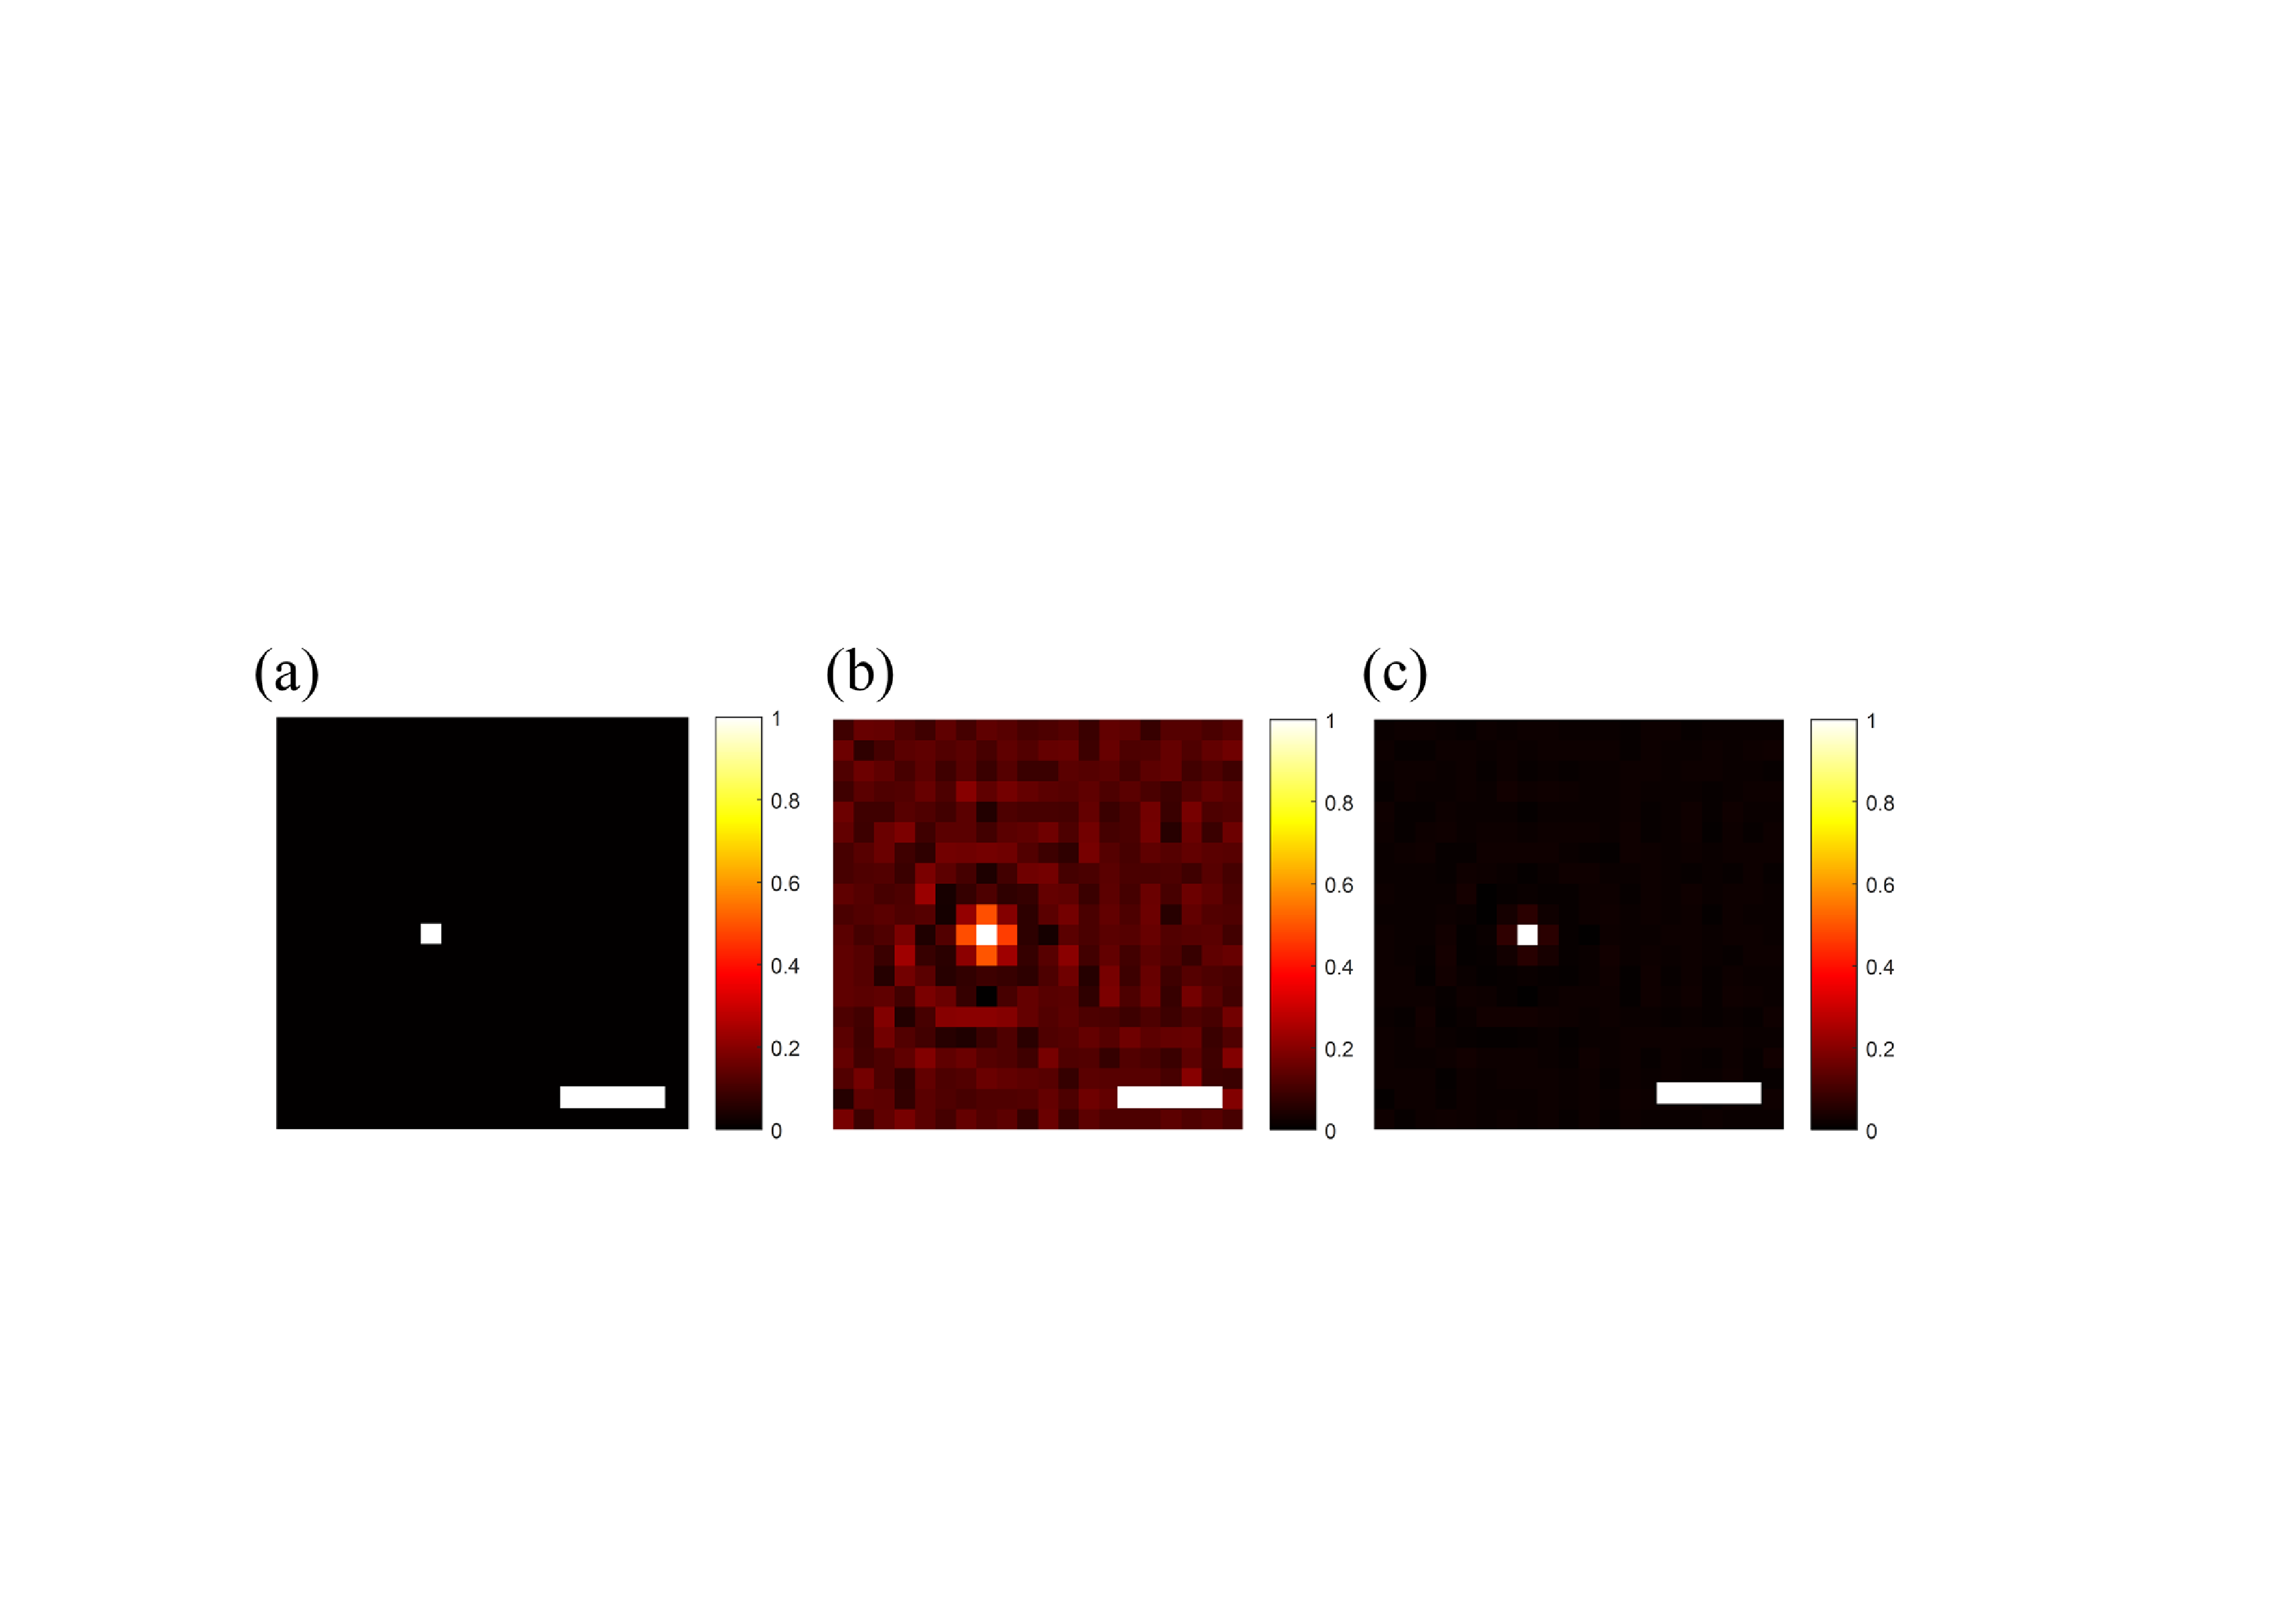
\includegraphics[scale=0.33]{C3.fig18.spectral_retrieval_model}
	\caption{点源目标的重建结果}
	\label{fig:3.18}
\end{figure}

为了更好地验证混合型非线性优化算法在基于SSTM透过散射介质成像应用的可行性和有效性,我们利用数字目标进行实验,并将基于矩阵求逆方法的实验结果和混合型非线性优化算法的实验结果进行了比较。实验结果如图\ref{fig:3.19}所示, 其中,混合型非线性优化算法的目标重建结果如图\ref{fig:3.19}(a2)所示, 利用矩阵求逆方法的目标重建结果如图\ref{fig:3.19}a3所示。图\ref{fig:3.19}(a4)定量比较了图\ref{fig:3.19}(a2)—\ref{fig:3.19}(a3)中两条虚线对应的强度分布。为了定量分析重建效果,我们将图像信噪比定义为:目标重建信号(原始目标对应的区域强度值)与背景噪声(除去目标区域的强度分布的平均值)之间的比值。经计算可得基于矩阵求逆的方法与非线性优化算法对应的信噪比分别为:3.3328和5.5669。由此说明,混合型非线性优化算法能够有效地抑制背景噪声,将信噪比提高1.7倍以上,更适合于基于SSTM的透过散射介质成像。图\ref{fig:3.19}(b)(\ref{fig:3.19}(c))与图\ref{fig:3.19}(a)相似,仅所采用的数字目标不同。

\begin{figure}[htp]
	\centering
	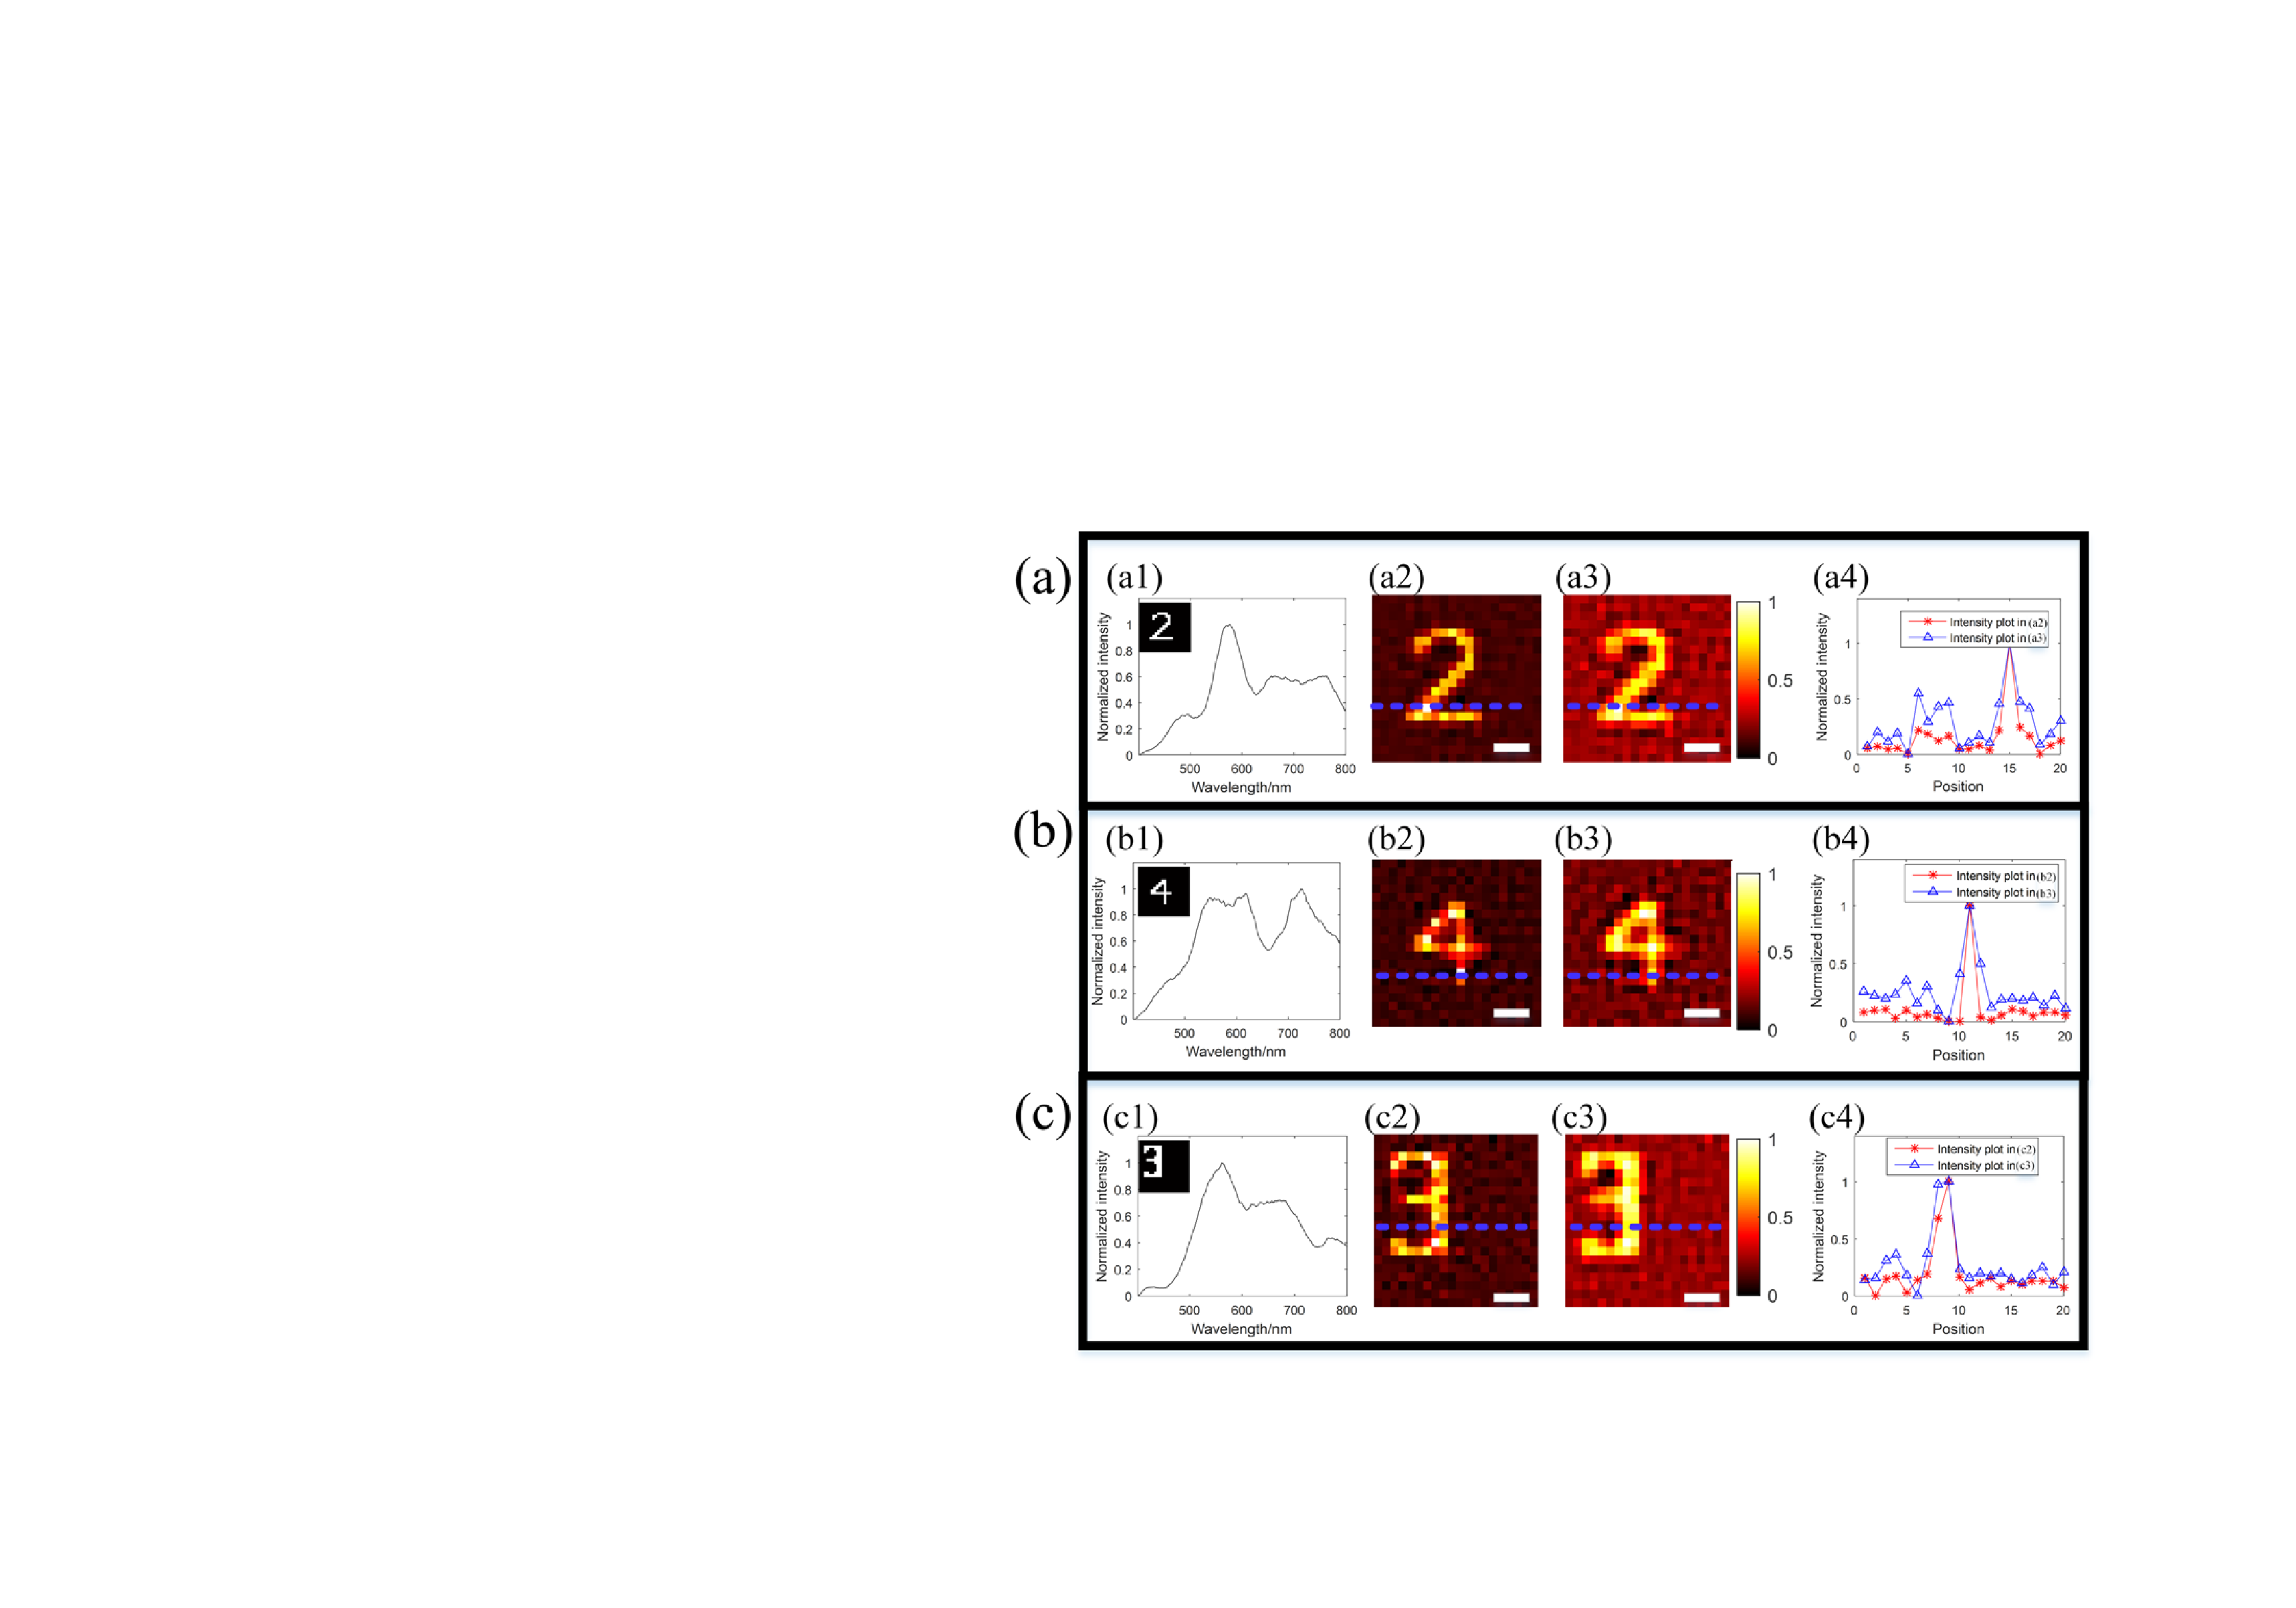
\includegraphics[scale=0.45]{C3.fig19.spectral_retrieval_model}
	\caption{数字目标的重建结果}
	\label{fig:3.19}
\end{figure}

基于SSTM的透过散射介质成像方法需要说明以下三点。 首先,与传统透过散射介质成像方法相比,该方法将SSTM与散射介质的色散特性相结合,实现了透过散射介质成像。传统光谱传输矩阵方法一直以来被用于光谱信号的重建。传统透过散射介质成像方法例如波前调制、光学相干层析、超快激光飞行时间成像法、散射矩阵测量和散斑相关等方法只适用单色光或者窄谱光源照明,而散射介质的光谱多样性被忽略。其次,该方法的视场和像距有一定的限制。因为散射介质的色散特性与散射介质的散射自由程有关,一般来说相距的选择主要考虑两方面因素:(\romannum{1})散斑场的分布特点和(\romannum{2})光谱信号的信噪比。当像面距散射介质距离较近时,未形成有效的散斑,光谱信号的位置多样性不能充分体现;当像面距散射介质距离较远时,光谱仪所接收到的光谱信号较弱、信噪比较低,对于目标重建和光谱传输矩阵测量都将引入误差,其FOV受到散射介质的光学特性、系统孔径和物面尺寸等多种因素的限制。

\section{讨论}

在本章前面的内容中,我们首先对绍了基于光谱传输矩阵的光谱重建方法和基于OME的散斑相关成像方法进行了介绍,并将其有机的结合,实现了利用散射介质的光谱信息恢复和目标恢复。然受,受到光谱传输矩阵方法的启发,我们将光谱传输矩阵的概念扩展到空间维度,实现了基于SSTM的透过散射介质成像。虽然透过数值仿真与实验验证,证明了以上方法的有效性,然而以上方法仍具有各自的局限性,具体如下:

(1)基于光谱传输矩阵的光谱重建方法

对于光谱矩阵的光谱重建方法而言,其核心在于对于系统的光谱传输矩阵预标定。在完成预标定之后,该方法的使用对系统的稳定性要求极其苛刻。而且,该方法的光谱分辨率受到散射介质的光谱去相关带宽限制。该方法的核心步骤为预标定,本质上记录了不同波长照明下各自的光谱指纹,而对于光谱指纹的选区不同也会对光谱重建的效果造成影响。当选取增大时,光谱的矩阵维度随之增加,但是光谱重建的精度提高;当选区减小时,其光谱重建的结果也会变差。不同的光谱重建算法,将会获得不同的的重建结果,如何选择合适的光谱重建优化算法也是未来亟待解决的问题之一。未来的潜在应用中,将光纤束作为散射介质,对其进行光谱传输矩阵标定,利用其实现光谱成像是潜在的应用的方法。但是其成像空间分辨将会受到单根光纤直径限制,其光谱分辨率会受到光纤长度的影响。

(2)基于OME的散斑相关成像方法

基于OME的散斑相关成像方法受限于OME的范围,当目标小于OME范围时,隐藏目标的傅里叶振幅能够通过散斑自相关方法有效的获取;但是当目标大于光学记忆相应范围时,该方法不能够有效的获取隐藏目标的傅里叶振幅信息。当不能获取隐藏目标的傅里叶振幅消息时,将无法利用前面小节所提到的相位恢复算法进行傅里叶相位恢复,因此导致无法恢复隐藏目标。当目标小于OME范围时,该方法仍有存在以下问题:其一,目前所使用的相位恢复算法通常采用随机相位作为相位恢复的初始猜测,当初始猜测不同时,可能导致不同的最终恢复结果。为了恢复到满意的结果,通常我们需要多次尝试,直至恢复到满意的结果,该恢复结果具有不确定性。其二,目前所采用的相位恢复算法,无法确定目标的方向信息,目标方向信息的丢失会影响该方法在更多场景下的应用。其三,该方法对目标的稀疏性有着严格的要求,通常难以实现连续的体目标进行成像,在成像过程中会丢失掉诸多细节信息。最后,该方法通过自相关的方式去除掉系统PSF的影响,然而系统PSF包含了系统的诸多特性,如果能够有效的利用PSF,将有助于更好的恢复目标信息。

(3)基于SSTM的透过散射介质成像方法

基于SSTM的散射成像方法受到散射介质的色散特性的影响,该方法需要进行预标定,无法对为标定的系统实现图像恢复。其成像分辨受到光谱仪分辨率的限制,也同时受到空间光谱多样性的限制。因此,该方法通常无法实现高分辨率或者复杂目标的成像。

\section{本章小结}

本章中我们首先对基于光谱传输矩阵的光谱重建模型和散斑相关成像的模型进行了介绍,它们分别被用来重建散斑的光谱信号和散斑所携带的隐藏目标的结构信息。我们对以上两种方法进行了有机的结合,利用散射介质实现了目标的结构信息恢复和光谱信息恢复,同时也进行了相应的实验,对以上方法进行实验验证。例如:我们通过实验证明了,当目标的照明光源为窄谱光源时,该方法能够有效的恢复目标的光谱信息和结构信息。随后,我们也实验验证了该方法对与宽谱光源照明时的有效性。同时,针对窄谱光源照明和宽谱光源照明时的结果差异进行了分析,得知当宽谱光源照明时,不同波长PSF之间的互相关项导致所恢复的隐藏目标的傅里叶振幅信息的准确度降低,进而造成重建结果的模糊。此外,我们受到光谱传输矩阵思想的启发,我对们SSTM方法进行了理论阐述,通过实验证明了基于SSTM的散射成像方法的有效性。最后,我们对本章中所涉及的三种方法的局限性,如:基于光谱传输矩阵的光谱重建方法受到预标定矩阵的影响,其光谱分辨率和光谱重建算的等问题;分析了基于光学记忆相应的散斑成像方法所存在的问题,其成像范围受到光学效应范围的影响,相位恢复算法所引入的重建不确定性,目标的分辨率问题。最后,我们也对基于SSTM的透过散射介质成像方法的限制进行了简单陈述。我们将会针对散斑相关成像的相位恢复问题展开工作,尝试在相位恢复过程中保存目标的相位信息。

在第四章中,受到天文成像中三阶相关的相位恢复方法的启发,将三阶相位相关的相位恢复算法应用到散斑相关成像中实现对隐藏目标的恢复。该方法能够有效的保持隐藏目标的方向信息,进而利用此特性实现了透过散射介质的彩色成像。
